\documentclass[pl]{minipw} % wszystkie ustawienia szablonu są w minipw.cls; if in English, change [pl] to [en]
\allowdisplaybreaks
\usepackage{indentfirst}
\usepackage{float}
\setlength{\parindent}{5mm} % wcięcie akapitowe 5mm, zarządzenie Rektora
\usepackage{hyperref}
\def\UrlBreaks{\do\/\do-}

% ------------ Ustawienia autora pracy ---------------

\setboolean{lady}{false} % kobiety wpisują true, mężczyźni - false

\title{Content-based recommendations in e-commerce services} % nazwa pracy
\titleaux{System rekomendacji artykułów opisujących produkty w serwisach e-commerce}
\type{magisters} % licencjat = licencjac, inżynier = inżyniers
\discipline{Informatyka} % kierunek
\specjal{Metody Sztucznej Inteligencji}
\author{Łukasz Dragan}
\album{254179}
\supervisor{dr~inż. Anna Wróblewska}
\date{2017}
\klucze{rekomendacje, przetwarzanie języka naturalnego, osadzanie słów, semantyka, allegro}
\keywords{recommendations, natural language processing, word embedding, semantics, allegro}
% ----------------------------------------------------

\begin{document}
\sloppy

% Nowy układ pracy dyplomowej

% 1. Strona tytułowa - trzeba wydrukować z osobnego pliku


% 2. Streszczenia
% Streszczenie ma zawierać tytuł pracy i słowa kluczowe
% if in English, English abstract goes first


\setcounter{page}{1}


\begin{streszczenie}

	Tematyka niniejszej pracy skupia się wokół zagadnień określania podobieństwa semantycznego pomiędzy dokumentami tekstowymi i rekomendacji dokumentów podobnych. Szczegółowy problem pochodzi z~internetowego serwisu aukcyjnego Allegro, który posiada dział artykułów opisujących produkty dostępne na~platformie. W~dziale tym funkcjonuje system rekomendacji podobnych artykułów tekstowych w~oparciu o~ich treść. Celem pracy jest zbadanie możliwości usprawnienia działania istniejącego systemu rekomendacji wykorzystując metody semantycznej analizy tekstu.
	
	W~niniejszej pracy adaptuję dostępne metody określania podobieństwa pomiędzy dokumentami tekstowymi do~powyższego problemu, wprowadzam miary umożliwiające ocenę działania tych metod oraz dokonuję analizy możliwości ich wykorzystania w~rzeczywistym systemie.
	
\end{streszczenie}


\begin{abstract}

	The subject of~this paper focuses on~issues of~determining the~semantic similarity between text documents and the~recommendation of~similar documents. A~detailed problem comes from~the~Allegro on-line auction site, which has a~section of~articles describing the~products available on~the~platform. This section offers a~recommendation system for~similar textual articles based on~their content. The~aim of~this paper is to~investigate the~possibility of~improving the~existing recommendation system using semantic text analysis methods.
	
	In~this paper, I adapt the~state-of-the-art methods for~determining the~similarity between text documents to~the~above problem, I introduce measures to~evaluate the~performance of~these methods and analyze the~possibilities of~using them in~the~real system.
	
\end{abstract}

% 2. Oświadczenie o autorstwie pracy - w innym pliku
\makestatement


% 4. Spis treści
\cleardoublepage
\tableofcontents

% 5. Treść

\cleardoublepage
\pagestyle{fancy}

\chapter*{Wstęp}
%TODO JAkie pytanie stawiam w pracy: czy semantyczne metody analizy języka naturalnego są w stanie dać lepsze efekty w zadaniu generowania rakomandacji od dotychczasowej metody stosowanej w Allegro opartej o silnik wyszukiwania Elasticearch i słowa kluczowe dobierane do artykułów przez ich autorów.
Systemy rekomendacji są powszechnym elementem wielu serwisów internetowych. Sprawdzają~się na~takich polach, jak polecanie produktów w~sklepie czy rekomendacje ofert pracy. Dają użytkownikowi poczucie indywidualnego traktowania przez serwis internetowy dopasowujący niejako zawartość swoich stron do~konkretnego użytkownika. Pozwala to użytkownikowi na~bardziej efektywne korzystanie z~serwisu oraz może prowadzić do~większego zaangażowania ze~strony użytkownika i przywiązania do~serwisu. Systemy rekomendacji dają obopólną korzyść zarówno użytkownikowi jak i właścicielowi serwisu internetowego.

Celem niniejszej pracy magisterskiej jest analiza możliwości usprawnienia istniejącego systemu rekomendacji w~oparciu o~adaptację istniejących metod wyszukiwania semantycznego podobieństwa pomiędzy dokumentami tekstowymi. Rzeczony system rekomendacji istnieje w~internetowym serwisie e-commerce Allegro w~dziale artykułów tekstowych o~tematyce związanej z produktami dostępnymi za~pośrednictwem serwisu. System ma na~celu zarekomendowanie użytkownikowi artykułów o~tematyce podobnej do~tego, który znajduje~się na~stronie aktualnie odwiedzanej przez użytkownika.

W~swojej pracy badam możliwość użycia istniejących metod semantycznej analizy tekstu w~odniesieniu do~opisanego problemu. Badane metody to: Latent Semantic Analysis, Latent Dirichlet Allocation, Word2vec, GloVe oraz FastText. Jakość działania tych metod porównuję poprzez samodzielnie opracowane metody ewaluacji.

Podczas prowadzenia badań stworzyłem szereg skryptów przetwarzających dane i~wykorzystujących implementacje opisywanych w~tej pracy metod. Opis użytych narzędzi programistycznych i~bibliotek zawarłem w~załączniku 1 do~niniejszej pracy. Stworzone skrypty umieszczam na~płycie CD dołączonej do~pracy. Opis zawartości płyty znajduje się w~załączniku 2.

\section{System rekomendacji artykułów tekstowych w Allegro}%DONE
Allegro jest największą \cite{all_naj} działającą na rynku polskim platformą aukcyjną on-line. Posiada ponad 20~milionów zarejestrowanych klientów. Każdego dnia na~Allegro sprzedaje~się ponad 870~tysięcy przedmiotów. Firma zatrudnia 1300 pracowników \cite{allegro}. Serwis umożliwia użytkownikom wystawianie na~sprzedaż oraz~kupno przedmiotów poprzez mechanizm licytacji lub~natychmiastowego zakupu.

Oprócz głównej części serwisu odpowiedzialnej za~transakcje, Allegro posiada dział zajmujący~się publikacją artykułów opisujących produkty wystawiane za~pośrednictwem serwisu. Ma to na~celu pomoc użytkownikom przy~wyborze interesującego ich produktu.

Po to, aby zachęcić użytkowników do~zapoznania się z~treścią kolejnych artykułów, zastosowany został tu system rekomendacji przyporządkowujący danemu artykułowi listę powiązanych artykułów. Kryterium mówiącym, czy artykuły są powiązane jest tutaj jedynie treść samych artykułów, a nie wcześniejsze zachowanie użytkownika.

\begin{figure}[H]
	\centering
	
\includegraphics[width=1\textwidth]{img/screen_allegro.png}
	\caption{Widok strony internetowej zawierającej jeden z artykułów serwisu Allegro \cite{screen_allegro}.}
\end{figure}

Od serwisu Allegro otrzymałem zserializowaną kopię 20000 artykułów dostępnych na~stronach serwisu. Pojedynczy artykuł składa się z~głównej zawartości tekstowej oraz metadanych. W~celu otrzymania wszelkich danych od~firmy Allegro wymagane było, abym podpisał umowę, w~której zobowiązuję się do nieujawniania żadnych danych, które otrzymałem. Stąd opisy danych, na których pracuję, zawarte w~tej pracy nie wnikają w~ich szczegóły i~nie odbiegają od~informacji publicznie dostępnych za~pośrednictwem strony pod~adresem \url{https://allegro.pl/artykuly}.

Aktualnie w~rzeczonym dziale serwisu Allegro istnieje system rekomendacyjny, który opiera~się o~wyszukiwanie podobnych artykułów tekstowych za~pomocą silnika Elasticsearch \cite{elastic}. Metoda ta wykorzystuje słowa kluczowe przypisane do~każdego artykułu przez~autora. W~swojej pracy staram~się porównać wyniki działania dotychczasowej metody z~metodami semantycznej analizy tekstu, które potrafią wykryć podobieństwo pomiędzy artykułami bazując jedynie na~ich treści, bez~potrzeby dołączania żadnych metadanych. Pomyślna próba zastosowania metod semantycznych pozwoliłaby na dokładniejsze dopasowanie podobnych artykułów w oparciu być może o~pewne ukryte cechy semantyczne nieosiągalne dla~silnika wyszukiwania tekstowego, jakim jest Elasticsearch. Bardziej szczegółowego opisu silnika Elasticsearch dokonuję w~kolejnym rozdziale.

\section{Struktura pracy}
W rozdziale 1 wprowadzam do zagadnienia systemów rekomendacji oraz~dokonuję przeglądu metod semantycznej analizy tekstu, które mogą zostać zastosowane w~celu określenia podobieństwa pomiędzy~dokumentami tekstowymi.

Następnie w~rozdziale 2 dokonuję opisu konkretnego problemu, jakim jest generacja rekomendacji artykułów tekstowych w~serwisie Allegro. Opisuję dane otrzymane~z serwisu oraz kolejne etapy ich wstępnego przetwarzania, aby nadawały~się do~zaaplikowania do~nich wybranych metod.

Dalej, w rozdziale 3 opisuję stworzone i~zastosowane później metody ewaluacji wyników.

Następnie, w~rozdziale 4 dokonuję opisu testów: jakie metody i~w~jaki sposób testuję.

W rozdziale 5 opisuję wyniki przeprowadzonych eksperymentów.

Ostatecznie w rozdziale 6 dokonuję podsumowania przeprowadzonych badań i~rozważam kierunki dalszych prac w~tej dziedzinie.

\section{Uwagi}
W~celu uniknięcia nieporozumień należy podkreślić różnicę pomiędzy znaczeniami słowa ,,artykuł'', które może oznaczać zarówno tekst publicystyczny, literacki lub naukowy jak~i~rzecz, która jest przedmiotem handlu \cite{slownik}. W~niniejszej pracy skupiam~się na~rekomendacjach artykułów tekstowych, stąd używam pierwszego znaczenia (chyba, że~inne znaczenie jest wyraźnie zaznaczone).

\chapter{Przegląd wiedzy z zakresu tematyki pracy}
W~swojej pracy dokonuję adaptacji metod przetwarzania języka naturalnego na~potrzeby generowania rekomendacji artykułów tekstowych w~oparciu o~ich treść. W~niniejszym rozdziale dokonuję przeglądu znanych metod z~obszaru tematyki pracy dyplomowej, skupiając~się szczególnie~na nowo powstałych metodach wektorowej reprezentacji słów, które cieszą~się obecnie dużym zainteresowaniem środowisk naukowych oraz firm komercyjnych. 

Dokonuję krótkiego wprowadzenia do~zagadnienia generowania rekomendacji, którego głęboka analiza nie jest konieczna z punktu widzenia niniejszej pracy. Następnie wykonuję chronologiczny przegląd metod ciągłej reprezentacji słów zaczynając od~trywialnych metod zliczania słów (bag-of-words, TF-IDF), przechodząc przez metody wykorzystujące koncepcję tematów (Latent Semantic Analysis, Latent Dirichlet Allocation) i~kończąc na~głośnych ostatnio metodach osadzania słów w przestrzeni wektorowej (Word2vec, GloVe, FastText). Przy~zarysie historycznym opieram~się w~dużej mierze na~artykule \cite{aylien}.

%Część z nich (metoda tf-idf, bag-of-words, silnik Elasticsearch oparty na indeksie Lucene\cite{lucene}) jest od lat powszechnie wykorzystywana w zadaniu wyszukiwania tekstowego. Inne z kolei - korzystające z semantycznej analizy tekstu - nie są tak popularne z powodu swojej nowości, bądź trudności w zaaplikowaniu. Daje to pole do badań i ewentualnych usprawnień istniejących systemów opierających się o klasyczne metody. Wybrane metody stosuję, zgodnie z tematem pracy, w zadaniu generowania rekomendacji, stąd przegląd metod zaczynam właśnie od wprowadzenia do tego zagadnienia.

\section{Systemy rekomendacji}

Systemy rekomendacji to narzędzia i~techniki mające na~celu zasugerowanie użytkownikowi przedmiotów. Sugestie te odnoszą~się do~różnych procesów podejmowania decyzji takich jak np. które artykuły kupić, jakiej muzyki słuchać czy też które wiadomości czytać. ,,Przedmiot'' jest tutaj ogólnym pojęciem oznaczającym coś, co system poleca użytkownikowi \cite{handbook}. 

Przy~wciąż wzrastającej ilości danych użytkownicy serwisów internetowych często nie są w~stanie dotrzeć do~informacji, która ich interesuje. Jest to pole do~rozwoju zautomatyzowanych systemów rekomendacyjnych polecających użytkownikom treści, które mogą ich zainteresować. Działalność takiego systemu daje zysk zarówno użytkownikowi, pozwalając mu dotrzeć do~informacji, której mógłby samodzielnie nie odszukać, albo wręcz nie wiedzieć, iż~taka informacja istnieje, jak~i~właścicielowi serwisu internetowego, któremu zależy, by przyciągnąć do~siebie użytkowników, aby ci w~jak~największym stopniu korzystali z~ich usług.

Sposoby działania systemów rekomendacji można podzielić na~różne warianty, spośród których wyodrębnić można dwa najszerzej używane. Są to: filtrowanie kolaboratywne (collaborative filtering) i~filtrowanie oparte na~treści (content-based filtering).

\subsection{Filtrowanie kolaboratywne (collaborative filtering)}
Technika ta opiera~się na~spostrzeżeniu, iż użytkownicy o~podobnych preferencjach zachowują się podobnie. Stąd jeżeli użytkownik zachowuje się podobnie do~zaobserwowanej wcześniej grupy użytkowników, można przewidzieć jego preferencje na~podstawie zachowań owej~grupy. Istotną zaletą tej metody jest fakt, iż nie~zależy ona od~dziedziny, w~której ulokowany jest system rekomendacji (w~przeciwieństwie do~rekomendacji opartych na treści), a~jedynie od~zachowań użytkowników.
\subsection{Filtrowanie oparte na treści (content-based filtering)}
W~technice tej przedmioty polecane użytkownikowi zależą od~innych przedmiotów, na~temat których stwierdzono, że użytkownik się nimi interesuje. Mogą~się one opierać np. na~podobieństwie przedmiotów: jeżeli użytkownik ,,lubi'' przedmiot $A$, który jest podobny do~przedmiotu $B$ to można spodziewać się, że również przedmiot $B$ zainteresuje użytkownika. Technika ta jest mocno zależna od~dziedziny rekomendowanych przedmiotów, gdyż wymaga wprowadzenia pewnej miary podobieństwa między nimi. Stąd jest trudniejsza do~zastosowania, ale daje też możliwości nieosiągalne dla~filtrowania kolaboratywnego.

Celem niniejszej pracy jest zbadanie metod sugerujących użytkownikowi artykuły podobne do~aktualnie odwiedzanego, co wprost wiąże się z~metodami używanymi w~technice filtrowania opartego na~treści.

\section{Silnik Elasticsearch}

Obecnie wykorzystywana przez Allegro metoda generowania rekomendacji artykułów opiera~się o~zapytanie do~usługi Elasticsearch \cite{elastic} wykorzystujące słowa kluczowe manualnie dołączone do~artykułów. Elasticsearch jest popularnym silnikiem wyszukiwania tekstu opartym o~indeks Lucene \cite{lucene}. Działa w~architekturze rozproszonej a~komunikacja z~nim następuje poprzez protokół HTTP i~format JSON. Umożliwia on efektywne przechowywanie dokumentów tekstowych oraz~efektywne ich wyszukiwanie. 

Apache Lucene jest biblioteką napisaną w~języku Java służącą do~wyszukiwania tekstu, która w~tym celu wykorzystuje mechanizm odwróconego indeksu. Zasada działania biblioteki polega na~stworzeniu słownika ze~wszystkich (odpowiednio wstępnie przetworzonych) słów dokumentów przeznaczonych do~wyszukiwania. Następnie na~bazie owego słownika tworzony jest odwrócony indeks. Każdemu ze słów przypisywana jest lista dokumentów, które zawierają to słowo. Pozwala to przyspieszyć proces wyszukiwania, gdyż w~poszukiwaniu pojedynczego słowa biblioteka nie~przeszukuje całego zbioru dokumentów, a~jedynie słownik, który na~ogół jest wielokrotnie krótszy.

Zaletą silnika Elasticsearch są jego wydajność, skalowalność, niezawodność i prostota użytkowania, co przekłada~się na~jego dużą popularność wśród np.~serwisów internetowych \cite{elastic_companies}.

Wadą metody jest to, że ogranicza się ona do wyszukiwania tekstowego pomijając aspekt semantyczny. Stwarza to trudności przy wyszukiwaniu synonimów lub homonimów.%Znaczy to, że jeżeli dwa teksty opisują ten sam temat, ale używają to tego różnych słów, np. synonimów, to systemowi opartemu jedynie o wyszukiwanie tekstowe nie uda się stwierdzić podobieństwa między tymi tekstami, mimo, iż takowe istnieje. Inną trudnością jest problem polisemii - sytuacji, gdy jedno słowo posiada dwa znaczenia (homonimy). Metoda  wyszuka wszystkie dokumenty je zawierające niezależnie od kontekstu, w jakim szuka ich użytkownik.


\section{Techniki przetwarzania języka naturalnego}
%TODO na końcu zreformatować cały rozdział, żeby zachować spójność formy opisu metod
Oparcie rekomendacji jedynie na treści artykułu wymaga zagłębienia się w tematykę analizy i przetwarzania języka naturalnego, wszak właśnie w języku naturalnym, zrozumiałym dla człowieka (polskim) pisane są owe artykuły. Język naturalny z powodu swojego niskiego stopnia sformalizowania nie jest niestety wprost zrozumiały dla maszyn. W związku z tym koniecznym staje się tu użycie technik przetwarzania języka naturalnego (natural language processing), które to pozwalają wyodrębnić z tekstu pewne cechy, na bazie których maszyna obliczeniowa przy pomocy pewnych algorytmów jest w stanie określić podobieństwo pomiędzy dokumentami. W poniższych paragrafach dokonuję przeglądu technik matematycznej reprezentacji dokumentów pisanych w języku naturalnym. Warto wspomnieć, iż dziedzina ta bardzo dynamicznie się rozwija, a część z opisywanych metod zostało stworzonych na przestrzeni ostatnich kilku lat, czy wręcz miesięcy.

W celu formalizacji w dalszych opisach stosowanych metod stosuję następujące oznaczenia:
\begin{itemize}
	\item Korpus $C$: zbiór dokumentów $d_i$,
	\item Dokument $d$: skończony ciąg zdań $s_i$,
	\item Słowo $w$: skończony ciąg znaków $c_i$,
	\item Słownik zbudowany na korpusie $C$: $V = \{w\ |\ \exists_{d \in C}\ w \in d\}$.
\end{itemize}

\subsection{Bag-of-words}
Bag-of-words (worek słów) \cite{bow} jest jedną z pierwszych koncepcji reprezentacji tekstu jako zbioru zawartych w nim słów w postaci wektorów. Metoda nie bierze pod uwagę kolejności słów w tekście, lecz liczbę ich wystąpień. Istotną zaletą reprezentacji wektorowej dokumentów jest możliwość zdefiniowania miary odległości pomiędzy dokumentami (np.~miara kosinusowa opisana później) odzwierciedlającej ich podobieństwo. Technikę tę można opisać jako przekształcenie z korpusu w przestrzeń wektorów $ bow: C \to \mathbb{R}^n $ gdzie:\\
$C$: korpus\\
$m = |C|$: liczba dokumentów w korpusie $C$\\
$V$: słownik zbudowany na $C$\\
$n = |V|$: liczba słów w $V$\\
$v_i \in \mathbb{R}^n$, gdzie $i \in 1, 2, ..., n$ wektor reprezentujący dokument $d_i \in C$\\
$v_{ij}$, gdzie $j \in 1, 2, ..., m$: liczba wystąpień w dokumencie  $d_i \in C$ słowa $w_j \in V$\\

Technika ta jest stosunkowo prosta, lecz jej wadą jest traktowanie każdego słowa z jednakową wagą. Pewne słowa (np.~,,i'', ,,lub'', ,,o'') występują bardzo często, lecz ich wkład w~znaczenie całego dokumentu jest marginalny. Stąd powstały bardziej zaawansowane techniki uwzględniające istotność słów dla znaczenia całego dokumentu. Mimo to metoda BOW jest często wykorzystywana w bardziej zaawansowanych technikach NLP, a także przy przetwarzaniu wstępnym tekstu przy okazji zadań usunięcia słów stopu oraz lematyzacji --- w celu zmniejszenia wymiarowości przestrzeni wektorowej słów.
\subsection{Term frequency - inverse document frequency}

TF-IDF \cite{tf_idf} (ważenie częstością termów - odwrotna częstość w dokumentach) jest metodą reprezentacji tekstu jako zbioru słów przy jednoczesnym uwzględnieniu wagi słów, która zależy od częstości występowania słowa w korpusie.  Oznaczenia formalne takie same tak w przypadku BOW.
$v_{ij} = tfidf_{ij} = tf_{ij} * idf_i$, gdzie:\\
$tf_{ij} = \frac{n_{ij}}{\sum\limits_{k}n_{kj}}$, ,,term frequency'' to liczba wystąpień słowa $w_i$ w dokumencie $d_j$ podzielona przez liczbę słów dokumentu $d_j$,\\
$idf_i = log\frac{|D|}{|{d:w_i \in d}|}$, ,,inverse document frequency'' to liczba dokumentów w korpusie podzielona przez liczbę dokumentów zawierających przynajmniej jedno wystąpienie słowa $w_i$,

Dokumenty reprezentowane są tu jako wektory, składające się z wag słów występujących w każdym z nich. TF-IDF przechowuje informację o częstotliwości występowania słów biorąc przy tym pod uwagę istotność znaczenia słowa lokalnego w stosunku do jego znaczenia w kontekście całego zbioru dokumentów. W tej technice słowa występujące rzadko są premiowane względem słów pospolitych. Wadą metody tej i poprzedniej jest postać wektorów reprezentujących słowa: są to na ogół rzadkie wektory dużej wymiarowości.

\subsection{Distributional semantics}
Kolejne, bardziej zaawansowane, omawiane tu metody opierają się na tzw. ,,distributional hypothesis'' - hipotezie zakładającej, że słowa występujące w tym samym kontekście niosą ze sobą podobne znaczenie\cite{bow}\cite{firth}. Sprzyja to zastosowaniu metod algebry liniowej jako narzędzia obliczeniowego oraz sposobu reprezentacji tekstu. Podstawowe podejście polega na zgromadzeniu informacji o rozkładzie słów w dokumentach w postaci wielowymiarowych wektorów a następnie wyodrębnieniu podobieństw pomiędzy tymi wektorami, które świadczyłyby o pewnych powiązaniach między reprezentowanymi słowami. 

\subsection{Latent Semantic Analysis}
%TODO przeczytać waziaka jeszcze raz
Analiza rozkładu słów w dokumentach tekstowych pozwala na wyodrębnienie podobieństw między słowami pod kątem: ich znaczenia (podobieństwo tematu słowa), ich osadzenia w stosunku do innych typów słów czy też ich struktury wewnętrznej. Dwie istotne metody: Latent Semantic Analysis \cite{lsa} oraz Latent Dirichlet Allocation \cite{lda} zakładają istnienie abstrakcyjnych niejawnych (latent) tematów, do których można przydzielić słowa wchodzące w skład korpusu.

LSA (1990) \cite{lsa}, znane również jako Latent Semantic Indexing (LSI) dokonuje transformacji każdego dokumentu w wektor dł. $|V|$ posiadający na $i$-tym miejscu wagę TF-IDF $i$-tego słowa ze słownika. W ten sposób tworzona jest rzadka macierz: kolumny reprezentują dokumenty a wiersze reprezentują unikalne słowa. W celu identyfikacji istotnych cech tej macierzy dokonuje się rozkładu według wartości osobliwych (Singular Value Decomposition\cite{svd}, SVD), który jest techniką redukcji wymiarowości. Celem użycia SVD jest redukcja liczby wierszy macierzy dla wydajniejszych dalszych obliczeń numerycznych oraz pozbycie się szumów, utrzymując jednocześnie podobieństwa pomiędzy kolumnami. Ostatecznie uzyskuje się macierz przynależności tematów do dokumentów, gdzie wiersze odpowiadające tematom można interpretować jako kombinacje pierwotnych wierszy-słów o podobnym znaczeniu. Np. $\{(samochod), (ciagnik), (jezdnia)\} \to \{(1.3452 * samochod + 0.2828 * ciagnik + 0.3 * jezdnia)\}$. Wymiar uzyskiwanej macierzy jest ustalany za pomocą hiperparametru, który oznacza liczbę tematów. Używając uzyskanej macierzy, podobieństwo pomiędzy kolumnami-dokumentami obliczane jest wykorzystując odległość kosinusową (opisaną później w tym rozdziale). Metoda LSA łagodzi problem synonimów poprzez scalanie podobnych słów w jeden temat. Niweluje również problem homonimów, włączając je częściowo w skład różnych tematów. Niemniej jednak poprzez arbitralne ustalanie hiperparametru odpowiedzialnego za liczbę tematów część semantycznie odrębnych tematów może zostać wchłonięta przez inne lub też rozbicie na tematy może być zbyt ,,drobne'' nie wykorzystując w pełni semantycznych powiązań.

%(2003)
%This means that if we have an LSI representation of a collection of documents, a new document not in the collection can be ``folded in'' to this representation using Equation 244. This allows us to incrementally add documents to an LSI representation. Of course, such incremental addition fails to capture the co-occurrences of the newly added documents (and even ignores any new terms they contain). As such, the quality of the LSI representation will degrade as more documents are added and will eventually require a recomputation of the LSI representation.

\subsection{Latent Dirichlet Allocation}

LDA \cite{lda} jest techniką automatycznego wykrywania niejawnych (\textit{latent}) tematów zawartych w dokumentach przy użyciu uczenia nienadzorowanego. LDA reprezentuje dokumenty jako mieszanki tematów, które z kolei reprezentowane są jako rozkłady prawdopodobieństwa na zbiorze słów. Liczba tematów ustalana jest za pomocą hiperparametru. LDA jest modelem statystycznym, który wykorzystuje m.in. rozkład Dirichleta. 

Rozkład Dirichleta to ciągły rozkład prawdopodobieństwa parametryzowany przez wektor $\alpha$ $K$ dodatnich liczb rzeczywistych. Wymiar wektora $\alpha$ określa wymiar rozkładu. Gęstość rozkładu Dirichleta wyraża się wzorem: $ f\left(x_{1},\cdots ,x_{K-1};\alpha _{1},\cdots ,\alpha _{K}\right)={\frac {1}{\mathrm {B} (\alpha )}}\prod _{i=1}^{K}x_{i}^{\alpha _{i}-1}$, gdzie $ x_{1},\cdots ,x_{K-1}>0$, $x_{1}+\cdots +x_{K-1}<1$, $x_{K}=1-x_{1}-\cdots -x_{K-1}$, a $B$ to stała normalizująca. Nośnikiem gęstości rozkładu jest $K-1$ wymiarowy sympleks.

W LDA rozkład Dirichleta jest wykorzystany w celu nadania początkowych wartości przynależności tematów do dokumentów oraz słów do tematów. Cechy rozkładu sprawiają, że tak dobrane początkowe wartości parametrów modelu są zgodne z intuicją, że dokument pokrywa jedynie mały zestaw tematów, a temat zawiera najczęściej tylko mały zestaw słów. Wykorzystanie rozkładu Dirichleta do określenia wartości początkowych skutkuje w rezultacie lepszym dopasowaniem dokumentów i tematów.

Przypuśćmy, że mamy zestaw dokumentów. Wybieramy ustaloną liczbę $T$ tematów, które zamierzamy wykryć. Chcemy użyć LDA w celu wyznaczenia reprezentacji każdego dokumentu jako mieszanki tematów oraz słów powiązanych z każdym tematem. Jednym ze sposobów, aby osiągnąć ten cel jest wnioskowanie oparte na próbkowaniu Gibbsa. Metoda ta działa zgodnie z następującymi krokami.

\begin{enumerate}
	\item Przejdź przez każdy dokument i losowo (zgodnie z rozkładem Dirichleta) przypisz każde słowo dokumentu do jednego z $T$ tematów.
	Warto zauważyć, iż etap ten daje pierwsze przybliżenie docelowej reprezentacji. W kolejnych krokach należy poprawiać to przybliżenie.
	\item Dla każdego dokumentu $d$, dla każdego słowa $w$ należącego do $d$, dla każdego tematu $t$ oblicz: $p(t | d)$, czyli odsetek liczby słów w $d$, które są aktualnie przypisane do tematu $t$ oraz oblicz $p(w | t)$, czyli odsetek liczby wystąpień słowa $w$, które są przypisane do tematu $t$ w skali całego korpusu. Przypisz słowu $w$ nowy temat poprzez losowanie z prawdopodobieństwem $p(t_i|d)*p(w|t)$ dla każdego tematu $t_i$.
\end{enumerate}
Ciągłe wykonywanie powyższych kroków doprowadzi do stabilnej sytuacji, w której przestaną następować zmiany przypisań słów do tematów. Wtedy należy zakończyć działanie algorytmu.

Zaletą LDA jest jego interpretowalność: do każdego tematu przypisane są z pewną wagą prawdziwe słowa pochodzące z przetwarzanego korpusu. Metoda ta może być traktowana jako technika redukcji wymiarowości, gdyż dopasowuje dokumentowi składającemu się z wielu słów reprezentację złożoną z małej liczby tematów.


\subsection{Word embeddings}
Od 2013r., wraz z wprowadzeniem przez T. Mikolova metody Word2vec \cite{word2vec} nastąpił gwałtowny rozwój i niewątpliwy sukces metod ,,word embeddings''. Określenie ,,word embeddings'' oznacza osadzanie słów w przestrzeni wektorowej przy pomocy uczenia nienadzorowanego i zostało po raz pierwszy użyte 2003r. w pracy Y. Bengio \cite{bengio}, gdzie wektory słów generowane są przez głęboką sieć neuronową. Ogół technik zaliczanych obecnie do ,,word embeddings'' cechuje się usiłowaniem reprezentacji słów wraz z zależnościami pomiędzy nimi w postaci wektorów o stosunkowo niskiej wymiarowości. Dzieje się to w opozycji do wcześniejszych podejść podobnych do bag-of-words - produkującego ogromne, rzadkie wektory, których wymiary równają się rozmiarowi słownika, o który oparty jest model (rzędu setek tysięcy). Ważną własnością metod osadzania słów jest zachowanie przez wektory semantycznych i syntaktycznych właściwości słów, co pozwala wykonywać na nich operacje artymetyczne na wektorach odwzorowujące cechy tychże słów np.~$vector("king")-vector("man")+vector("woman") \approx vector("queen")$ 

Stosowane obecnie podejścia generowania wektorowych reprezentacji słów można podzielić na dwa typy:
\begin{enumerate}
	\item Modele predykcyjne: uczą się wektorowych reprezentacji słów poprzez zmniejszenie błędu predykcji słów należących do lokalnego kontekstu słowa $i$. Poniżej opisuję sztandarowy przykład takiego modelu - Word2vec, gdzie sposobem na optymalizację funkcji celu jest zastosowanie płytkiej sieci neuronowej typu feed-forward optymalizowanej za pomocą metody stochastic gradient descent.
	\item Metody oparte o zliczanie: generują wektory słów poprzez redukcję wymiarowości w globalnej macierzy współwystąpień słów.
	Jako pierwszy etap konstruują one ogromną (wymiar równa się liczbie słów w słowniku korpusu) macierz, która (podobnie, jak  metodzie LSI) następnie ulega faktoryzacji, aby uzyskać macierz o mniejszym wymiarze, lecz nadal zachowującą powiązania pomiędzy słowami. Przykładem jest tu opisana poniżej metoda Global Vectors - GloVe.
\end{enumerate}

Jedną z szerokiego wachlarza możliwości, jakie dają tego typu techniki jest określanie podobieństwa pomiędzy całymi dokumentami, wykorzystując dodatkowe metody pozwalające przenieść zależności między poszczególnymi słowami dokumentu na zależności między całymi zbiorami słów, co jest istotne z punktu widzenia tematu niniejszej pracy. Dwie z nich: metodę centroidu oraz Word Mover's Distance opisuję później w tym rozdziale. Warto zauważyć, iż posiadając wektorową reprezentację słów można wyznaczyć ,,odległość'' pomiędzy dwoma dokumentami nawet, jeżeli nie posiadają one wspólnych słów.


\subsection{Podejścia deep learningowe}

Wspomniane podejście Bengio oparte jest o sieć neuronową typu feed-forward o jednej warstwie ukrytej zgodnie z architekturą z poniższego rysunku.

\begin{figure}[H]
	\centering
	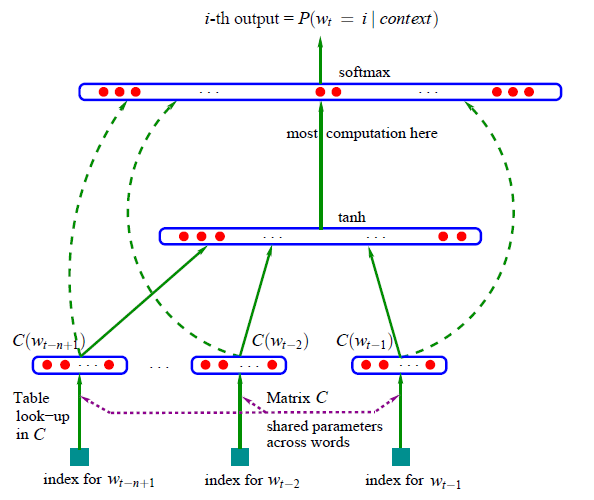
\includegraphics[width=1\textwidth]{img/bengio_language_model.png}
	\caption{Neuronowy model języka. Źródło: \cite{bengio}.}
\end{figure}

Celem działania sieci jest maksymalizacja funkcji celu $J_\theta = \frac{1}{T}\sum\limits_{t=1}^T\ \text{log} \space f(w_t , w_{t-1} , \cdots , w_{t-n+1})$, gdzie $f(w_t , w_{t-1} , \cdots , w_{t-n+1})$ odpowiada prawdopodobieństwu $p(w_t \: | \: w_{t-1} , \cdots , w_{t-n+1})$ wystąpienia słowa $w_t$ bezpośrednio po sekwencji słów $w_{t-1} , \cdots , w_{t-n+1}$. Wektorowa reprezentacja słowa uzyskiwana jest tu przez przemnożenie wejściowego wektora (wektor zer z jedynką na $i$-tym miejscu reprezentujący $i$-te słowo, ,,one-hot-vector'') z macierzą wag pierwszej warstwy sieci.


Podejście to jak i kolejne (\cite{c_w}) wykorzystujące głębokie sieci neuronowe nie znalazły zastosowań komercyjnych, ponieważ ich wydajność nauki jest na tyle  niska, że niemożliwe jest użycie przy ogromnych zbiorach danych wykorzystywanych w środowiskach produkcyjnych.


Rozwiązaniem tego problemu wydają się być nowe metody wektorowej reprezentacji słów powstałe na przestrzeni ostatnich lat. W odróżnieniu do metod deep learningowych opierają się one o metody szybkiej nauki, np.~o~płytkie sieci neuronowe, które uczą się na tyle krótko, że sprawdzają się one w zastosowaniach komercyjnych.


\subsection{Word2vec}%TODO przepisać rozdział tak, by był spójny z poprzednimi

Metoda Word2vec wprowadzona w 2013r. m.in. przez T. Mikolova w \cite{word2vec} odniosła niewątpliwy sukces w porównaniu z wcześniejszymi metodami osadzania słów w przestrzeni wektorowej. Autorzy metody proponują sieć neuronową, która podobnie jak wcześniejsze podejścia ma za zadanie odtworzyć kontekst danego słowa i na tej podstawie dokonać reprezentacji słowa jako wektora liczb rzeczywistych. Różnica jest taka, iż sieć ta ani nie jest głęboka, ani też nie zawiera nieliniowych funkcji aktywacji wykorzystywanej przy warstwie we wcześniejszych modelach. Wyróżnia się dwie odwrotne architektury sieci:
\begin{itemize}
	\item CBOW (continuous bag-of-words): na postawie okna $N$ sąsiednich słów sieć przewiduje słowo, którego z największym prawdopodobieństwem te $N$ słów jest sąsiedztwem. W tym modelu funkcja celu przyjmuje postać $J_\theta = \frac{1}{T}\sum\limits_{t=1}^T\ \sum\limits_{-n \leq j \leq n , \neq 0} \text{log} \space p(w_{t+j} \: | \: w_t)$.
	\item skip-gram: na podstawie słowa sieć dokonuje predykcji $N$ sąsiednich słów. Zadaniem sieci neuronowej jest wtedy optymalizacja funkcji celu postaci $J_\theta = \frac{1}{T}\sum\limits_{t=1}^T\ \text{log} \space p(w_t \: | \: w_{t-n} , \cdots , w_{t-1}, w_{t+1}, \cdots , w_{t+n})$.
\end{itemize}

\begin{figure}[H]
	\centering
	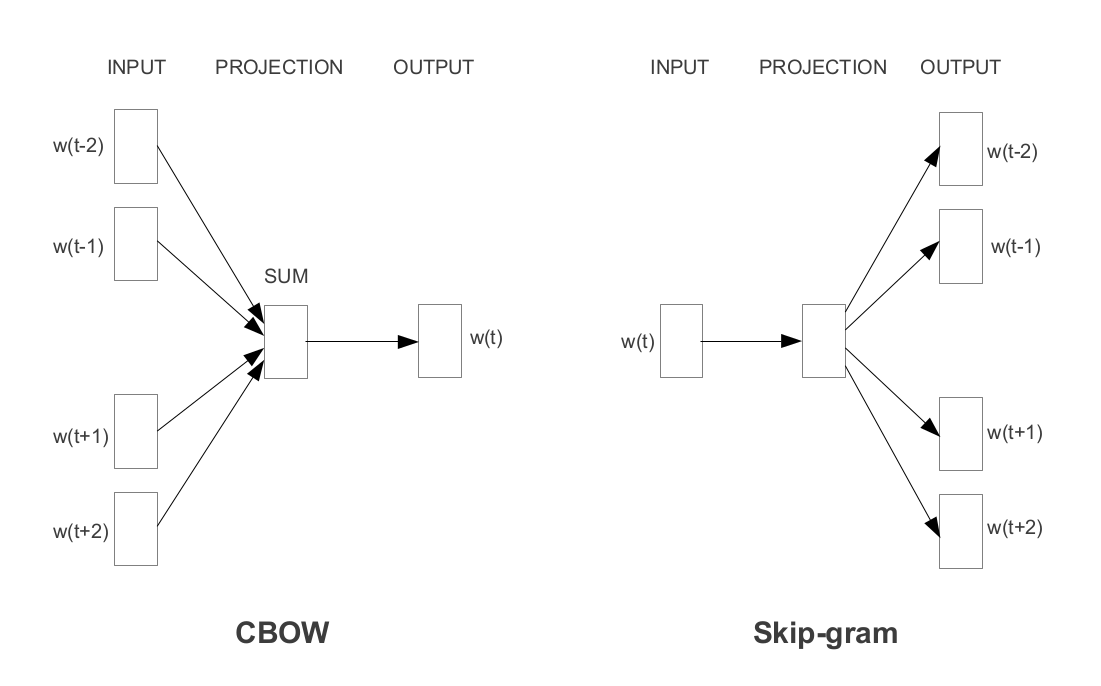
\includegraphics[width=1\textwidth]{img/skipgram_cbow.png}
	\caption{Schemat sieci wykorzystującej podejście skip-gram i CBOW. Źródło: \cite{word2vec}.}
	%\label{fig:warstwy}
\end{figure}
Używając tej stosunkowo prostej architektury można wykonać proces nauki używając milionów słów, których powiązania między sobą zostaną zachowane w systemie wag sieci neuronowej. Zaletą podejścia skip-gram są lepsze wyniki w przypadku rzadkich słów. Nauka w przypadku tego podejścia jest jednak wolniejsza niż w przypadku CBOW \cite{google_word2vec}.

W celu dalszego opisu metody Word2vec wprowadzam pojęcie funkcji softmax użytej w warstwie wyjściowej sieci neuronowej. Softmax jest generalizacją funkcji logistycznej, zamieniającą $K$-wymiarowy wektor $z$ dowolnych liczb rzeczywistych na $K$-wymiarowy wektor liczb rzeczywistych z zakresu $(0,1]$, które sumują się do $1$. Funkcja wyraża się wzorem $\sigma (\mathbf {z} )_{j}={\frac {e^{z_{j}}}{\sum _{k=1}^{K}e^{z_{k}}}}\ dla\ j=1,\ ...,K$. Wyjście funkcji można traktować jako pewien rozkład prawdopodobieństwa.

W metodzie Word2vec nauka polega na trenowaniu sieci neuronowej. Jednakże w odróżnieniu od innych metod wykorzystujących sieci neuronowe, Word2vec nie używa później wytrenowanej sieci jako takiej, a jedynie otrzymanych w wyniku nauki wag warstwy ukrytej sieci, które faktycznie są wynikowymi wektorami słów.

W dalszym opisie metody szczegółowo skupiam się na podejściu CBOW, lecz podejście skip-gram wygląda analogicznie.

Sieć neuronowa będąca wynikiem nauki przyjmuje na wejściu wektor binarny długości odpowiadającej liczbie słów w słowniku V zbudowanym na korpusie treningowym. Wektor ten wypełniony jest wartościami 0 oraz jedną wartością 1 na i-tej pozycji. Taki wektor odpowiada i-temu słowu ze słownika V. Wejściem sieci są kolejne słowa z korpusu w tej właśnie reprezentacji. Wyjściem sieci jest wektor tej samej długości o wartościach rzeczywistych z zakresu [0,1], w którym wartość na i-tej pozycji odpowiada prawdopodobieństwu, że i-te słowo ze słownika znajduje się w sąsiedztwie słowa wejściowego. Za ,,sąsiedztwo'' wielkości x należy tu rozumieć zbiór złożony z x słów występujących przed danym słowem w korpusie i x słów położonych za danym słowem. Wartość x może być tu ograniczona przez początek/koniec zdania, które ograniczają kontekst danego słowa.

Jako efekt należy~się spodziewać, że dla~słowa wejściowego ,,Brytania'' otrzymamy na~wyjściu wysoką wartość prawdopodobieństwa dla słowa ,,Wielka'', a~niską np.~dla~słowa ,,skoroszyt''.

Jednym z~parametrów metody Word2vec jest wymiarowość przestrzeni, w której znajdują się otrzymane wektory odpowiadające słowom z korpusu. Liczba ta ma swoje źródło z wielkości warstwy ukrytej sieci neuronowej. Wagi warstwy ukrytej można interpretować jako macierz $M$x$N$, gdzie $M$ to liczba słów słownika $V$ - wielkość wektora wejściowego, a $N$ to liczba neuronów w warstwie ukrytej. Po przeprowadzeniu nauki $i$-ty wiersz tej macierzy odpowiada wektorowi długości $N$, który reprezentuje $i$-te słowo ze słownika $V$.

W sieci nie jest używana funkcja aktywacji, ale prawdopodobieństwa na wyjściu są efektem działania funkcji softmax. Funkcja ta ma za zadanie sprowadzić wyjściowe wartości warstwy ukrytej do postaci rozkładu prawdopodobieństwa. 


\subsection{FastText}

FastText \cite{fasttext} to biblioteka stworzona w 2016 w celu wydajnego uczenia wektorowej reprezentacji słów oraz klasyfikacji zdań. Od ,,klasycznego'' Word2vec różni się stopniem szczegółowości analizy słów. Word2vec traktuje słowo jaką najmniejszą, niepodzielną jednostkę, której wektorową reprezentację usiłuje wyznaczyć. FastText natomiast dokonuje analizy również wewnętrznej analizy słów. Wykorzystuje w tym celu rozbicie słowa na podsłowa - ciągi znaków o określonej długości $n$, ,,character n-grams''. Np. słowo ,,pokój'' składa się następujących 3-gramów: [pok], [okó], [kój]. Podejście takie daje szereg nowych możliwości. Pomaga wyznaczyć reprezentację wektorową rzadkich słów, które być może mają wspólny rdzeń (i znaczenie) z innymi, częściej występującymi słowami. Metoda pozwala również nadać wektorową reprezentację słowom, których w ogóle nie ma w słowniku, jako że ich podsłowa mogą należeć do słów w słowniku się znajdujących. Zalety te wydają się być szczególnie obiecujące w przypadku bogatych morfologicznie języków, np.~języka polskiego, tureckiego, czy fińskiego.

Zasada działania metody bazuje na Word2vec. Jednakże oprócz predykcji tylko całych słów następuje tu również predykcja n-gramów słowa $a$ w otoczeniu słowa $a$. Ostatecznie słowu $a$ zostaje przypisany wektor składający się ze średniej oryginalnej reprezentacji wektorowej słowa oraz reprezentacji jego n-gramów.

Jak pokazuje badanie\cite{fast_text_word2vec} metoda ta sprawdza się lepiej od Word2vec w wykrywaniu syntaktycznych podobieństw pomiędzy słowami. 

\subsection{GloVe}

GloVe\cite{glove} (GLObal VEctors) jest kolejną wartą uwagi metodą word embedding powstałą na przestrzeni ostatnich lat. Algorytm GloVe różni się od Word2vec w sposobie uzyskania wektorowej reprezentacji słów. Word2vec jest modelem predykcyjnym, natomiast trening w GloVe opiera się na globalnej macierzy współwystąpień słów. Ponadto, w~porównaniu do~Word2vec, GloVe stara~się wyznaczyć reprezentacje wektorowe wprost, podczas gdy w~Word2vec dzieje~się ,,przy okazji'' - szkoli się sieć neuronową nie w celu jej dalszego wykorzystania w celu predykcji, a jedynie dla jej macierzy wag. 

Algorytm GloVe składa się z następujących kroków\cite{glove_cran}:
\begin{enumerate}
	\item Zgromadź współwystąpienia słów w formie macierzy $X$. Każdy element $X_{ij}$ takiej macierzy reprezentuje jak często słowo $i$ występuje w pobliżu słowa $j$. Zazwyczaj macierz buduje się poprzez skanowanie bazowego korpusu oknem o ustalonej szerokości, w obrębie którego centralne słowo leży w kontekście słów je otaczających. Dodatkowo można tu wprowadzić wagi dla słów malejące wraz ze wzrostem dystansu od słowa centralnego.
	\item Zdefiniuj ograniczenie dla każdej pary słów: $w_i^Tw_j + b_i + b_j = log(X_{ij})$, gdzie $w_i$ oznacza wektor głównego słowa, $w_j$ słowa leżącego w pobliżu $i$, $b_i$ i $b_j$ to skalary.
	\item Zdefiniuj funkcję kosztu $J = \sum_{i=1}^V \sum_{j=1}^V \; f(X_{ij}) ( w_i^T w_j + b_i + b_j - \log X_{ij})^2$, gdzie f jest funkcją ważącą, która pomaga zapobiec uczeniu tylko na podstawie najbardziej popularnych par słów. Autorzy proponują funkcję postaci:
	$f(X_{ij}) = 
	\begin{cases}
	(\frac{X_{ij}}{x_{max}})^\alpha & \text{if } X_{ij} < XMAX \\
	1 & \text{otherwise}
	\end{cases}$
	Celem funkcji optymalizacji funkcji	 kosztu jest minimalizacja różnicy pomiędzy iloczynami skalarnymi wektorów współwystępujących słów.
	\item Dokonaj minimalizacji funkcji kosztu poprzez stopniową aktualizację wektorów $w_i$ i $w_j$.
\end{enumerate}

\subsection{Odległość między dokumentami}
W celu wykorzystania omówionych metod osadzania słów, należy wybrać metodę obliczania odległości między całymi dokumentami, których słowa potrafimy reprezentować jako wektory. Zakładamy, że jeżeli dystans pomiędzy dokumentami jest mały, to ich tematyka jest podobna.
\subsubsection{Centroid}
Najprostszą i najbardziej intuicyjną metodą obliczenia odległości pomiędzy wektorową reprezentacją dokumentów jest wykonanie dwóch prostych kroków:
\begin{enumerate}
	\item Uśrednienie wektorów wchodzących w skład każdego z dokumentów. Powstały w ten sposób wektor jest centroidem reprezentującym dokument w przestrzeni wektorowej.
	\item Obliczenie dystansu między wektorami. Powszechnie przyjętą praktyką jest stosowanie tzw. odległości kosinusowej - znormalizowanego iloczynu skalarnego wektorów $A$ i $B$. Jest to kosinus kąta pomiędzy dwoma wektorami reprezentującymi dokumenty. Zaletą tej metody jest natychmiastowa normalizacja wyniku do zakresu $(0, 1)$. Odległość $sim={\mathbf {A} \cdot \mathbf {B}  \over \|\mathbf {A} \|_{2}\|\mathbf {B} \|_{2}}={\frac {\sum \limits _{i=1}^{n}{A_{i}B_{i}}}{{\sqrt {\sum \limits _{i=1}^{n}{A_{i}^{2}}}}{\sqrt {\sum \limits _{i=1}^{n}{B_{i}^{2}}}}}}$,
	gdzie $A_i$ i $B_i$ są składowymi wektorów odpowiednio $A$ i $B$
\end{enumerate}
Wadą opisanej powyżej metody jest utrata potencjalnie użytecznych zależności pomiędzy poszczególnymi wektorami wchodzącymi w skład dokumentu.

W kontrze do tego prezentuję metodę obliczania dystansu między dokumentami uwzględniającą rozkład wektorów wewnątrz dokumentu.

\subsubsection{Word Mover's Distance}
Word Mover's Distance \cite{wmd} to rozwiązanie zwracające odległość między dokumentami tekstowymi. W tym celu adaptuje algorytm Earth Mover's Distance \cite{emd} oraz wektorową reprezentację słów dokumentu. WMD mierzy odległość między dokumentami jako minimalny dystans jaki wektory słów pierwszego dokumentu muszą ,,pokonać'' aby osiągnąć wartości wektorów z drugiego dokumentu.

EMD jest metodą mierzenia odległości pomiędzy dwoma rozkładami, która opiera się na minimalnym koszcie, jaki musi zostać poniesiony, aby dokonać transformacji jednego rozkładu w drugi. Problem można sformalizować jako problem programowania liniowego, gdzie:
$P=\{f(p_1,w_{p_1})...(p_m,w_{p_m})\}$, $Q=\{f(q_1,w_{q_1})...(q_n,w_{q_n})\}$ są danymi rozkładami o $m$ (odpowiednio $n$) klastrach $p_i$ ($q_j$), a $w_{p_i}$ ($w_{q_j}$) jest masą klastra. $D=[d_{ij}]$ jest macierzą odległości, w której $d_{ij}$ reprezentuje odległość pomiędzy klastrami $p_i$ i $q_j$. Celem jest znaleźć taki przepływ $F = [f_{ij}]$, gdzie $f_{ij}$ to przepływ pomiędzy $p_i$ i $q_j$, który minimalizuje całościowy koszt $Work(P, Q, F) = \sum_{i=1}^{m}\sum_{n}^{j=1}d_{ij}f_{ij}$ przy odpowiednich ograniczeniach\cite{emd}.
EMD jest to dobrze zbadanym problemem transportowym \cite{emd}, dla którego powstały efektywne metody rozwiązania \cite{emd_method}. 

Przypuśćmy, że dzięki metodzie Word2vec dla słownika $V$ o $n$ słowach otrzymujemy macierz $X \in \mathbb{R}^{d \times n}$. $i$-ta kolumna tej macierzy reprezentuje $i$-te słowo ze słownika $V$. Odległości pomiędzy wektorami reprezentującymi semantycznie zbliżone słowa są relatywnie mniejsze od odległości dla słów niezwiązanych ze sobą. Celem WMD jest zawrzeć semantyczne podobieństwo pomiędzy poszczególnymi parami słów w dystans pomiędzy całymi dokumentami. Aby to osiągnąć metoda traktuje dokument jako rozkład, którego $i$-tym elementem jest liczba wystąpień $i$-tego słowa w tym dokumencie, a następnie stosuje metodę EMD do obliczenia dystansu między tymi rozkładami. Macierz odległości $D$ używana w metodzie EMD jest zbudowana na bazie odległości między wektorami Word2vec reprezentującymi słowa dokumentów. $d_{ij} = ||x_i-x_j||$, gdzie $i$ i $j$ to indeksy słów ze słownika $V$ a $x_{ij}$ to element macierzy $X$. Autorzy metody określają złożoność metody jako $O(p^3\log p)$, gdzie $p$ to wielkość słownika $V$.

\section{Miary oceny wyszukiwania}
%TODO przeredagować - to jest tekst ze slajdów

Razem z rozwojem systemów wyszukiwania informacji powstały miary pozwalające ocenić wyniki działania tych systemów. Do najbardziej popularnych należą ,,precyzja'' i ,,zwrot''.

Precyzja to odsetek wyszukanych dokumentów, które są relewantne do zapytania; $precision=\frac{|\{relevant\} \cap \{retrieved\}|}{|\{retrieved\}|}$.

Zwrot natomiast jest liczbą wyszukanych relewantnych dokumentów w stosunku do wszystkich relewantnych dokumentów (również tych niewyszukanych); $recall=\frac{|\{relevant\} \cap \{retrieved\}|}{|\{relevant\}|}$.

Bardziej złożoną miarą lepiej charakteryzującą jakość procesu wyszukiwania jest F-miara. W celu obliczenia wyniku uwzględnia ona zarówno precyzję jak i zwrot. Miara wyraża się wzorem: $F_\beta = (1 + \beta^2) \cdot \frac{\mathrm{precision} \cdot \mathrm{recall}}{(\beta^2 \cdot \mathrm{precision}) + \mathrm{recall}}$ Rezultat miary można interpretować jako ważoną średnią precyzji i zwrotu. 

Powyższe miary dokonują binarnego podziału wyników wyszukiwania: na relewantne i nierelewantne. Jednakże część rekomendowanych przedmiotów może być mniej lub bardziej od innych istotnych dla użytkownika. W tym świetle listę rekomendacji można uznać za pewien ranking, którego elementy mogą być uszeregowane lepiej lub gorzej. Ocena, czy dane uszeregowanie jest dobre, jest istotnym problemem z punktu widzenia ewaluacji metod generujących elementy rankingu. Stąd zachodzi potrzeba wprowadzenia formalnej miary jakości uszeregowania elementów rankingu. Można osiągnąć poprzez rozszerzenie podstawowych metod ewaluacji opartych na binarnej ocenie relewantności, jak recall i precision.

Miara nDCG \cite{ndcg} (Normalized Discounted Cumulative Gain) jest miarą jakości rankingu, która opiera się na założeniu, że im bardziej relewantne wyniki, tym wyżej powinny być w rankingu, aby ranking był najbardziej wartościowy. Miara ta mierzy skumulowany ,,zysk'' powstały poprzez umieszczenie poszczególnych przedmiotów na określonych pozycjach rankingu. Miara nDCG jest znormalizowaną wersją miary DCG (Discounted Cumulative Gain), która wyraża się wzorem: ${\mathrm  {DCG_{{p}}}}=\sum _{{i=1}}^{{p}}{\frac  {2^{{rel_{{i}}}}-1}{\log _{{2}}(i+1)}}$, gdzie $p$ to liczba elementów rankingu, $i$ to miejsce przedmiotu w rankingu, a $rel$ to poziom relewantności elementu. DCG premiuje relewantne przedmioty, które są wysoko w rankingu oraz karze za relewantne przedmioty w dole rankingu. W wariancie nDCG następuje jeszcze normalizacja przez podzielenie wartości DCG rzeczywistego rankingu przez DCG idealnego rankingu zbudowanego na elementach korpusu ułożonych malejąco pod kątem relewantności: ${\mathrm  {nDCG_{{p}}}}={\frac  {DCG_{{p}}}{IDCG_{{p}}}}$, $\mathrm {IDCG_{p}} =\sum _{i=1}^{|REL|}{\frac {2^{rel_{i}}-1}{\log _{2}(i+1)}}$, gdzie $REL$ oznacza listę relewantnych przedmiotów z całego zbioru podlegającego szeregowaniu.

\chapter{Dane}

Dane, na których testowane były opisywane w niniejszej pracy metody otrzymałem dzięki życzliwości serwisu Allegro. Jednak, by dane te otrzymać, zobowiązany zostałem po podpisania umowy o poufności. Stąd, w niniejszej pracy brak jakichkolwiek przykładów danych poza tymi dostępnymi za pośrednictwem strony internetowej Allegro. W niniejszym rozdziale opisuję strukturę i stan pozyskanych danych oraz proces ich wstępnego przetwarzania i analizy w celu zastosowania na nich zaadaptowanych metod opisanych w rozdziale poprzednim. 

\section{Opis danych}

Otrzymane dane to baza ok. 20000 artykułów tekstowych w formacie JSON. Są to te same artykuły, które są dostępne dla użytkowników poprzez serwis internetowy (stan na styczeń 2017). Pojedynczy rekord danych składa się z głównej treści artykułu oraz z metadanych, z których za istotne z punktu widzenia tematu pracy uznałem pola: id, kategoria i słowa kluczowe.

\subsection{Treść artykułu}

Treść każdego artykułu składa się z trzech pól: ,,zawartość'', ,,nagłówek'' i ,,tytuł''. Średnia długość artykułu to 821 słów, w tym nagłówek to jednozdaniowy wstęp. Średnią tę estymuję na podstawie średniej liczby znaków artykułu i średniej długości słowa w języku polskim. Dokładne statystyki tekstu będą dostępne dopiero po wstępnym przetwarzaniu.

Wszystkie artykuły napisane są w języku polskim, w nielicznych przypadkach wykryłem błędy, tzw. ,,literówki''. Jako, że artykuły ze zbioru dotyczą produktów sprzedawanych za pośrednictwem serwisu Allegro, w skład słownika zbudowanego na ich bazie wchodzi wiele słów specyficznych dla różnych branż. Są to m.in. nazwy modeli aparatów (np.~,,Sony Alpha 77 II''), samochodów, gier komputerowych, a także nazwy techniczne: ,,sprężarka'', ,,hipertoniczny'', ,,autofocus''.

Artykuły posiadają w swej treści wiele znaczników interpretowanych przez system, na podstawie których wzbogacana jest warstwa wizualna strony internetowej zawierającej artykuł, np.~obrazki czy łącza do ofert związanych z tematem artykułu.

Spójność danych oceniam na wysoką, tj. każde pole zawarte w strukturze dokumentu jest zawsze wypełnione - brak jest wartości typu NULL.

\subsection{Kategoria}

Każdy artykuł został przez autora przydzielony do pewnej kategorii, która odpowiada tematyce artykułu, np.~,,Aparaty cyfrowe'' czy ,,Przyprawy i zioła''. W skład pola ,,kategoria'' wchodzi również lista kategorii nadrzędnych, a cała hierarcha kategorii ma strukturę drzewiastą. Np. kategoria nadrzędna dla kat. ,,Przyprawy i zioła'' to ,,Delikatesy'', a dla kat. ,,Delikatesy'' to  ,,Dom i zdrowie''. Każdy artykuł należy do tylko jednej kategorii będącej dowolnym węzłem w drzewie (nie tylko liściem). Drzewo kategorii posiada 8 poziomów, a najwięcej węzłów znajduje się na poziomach 5 i 6. 
\begin{figure}[H]
	\centering
	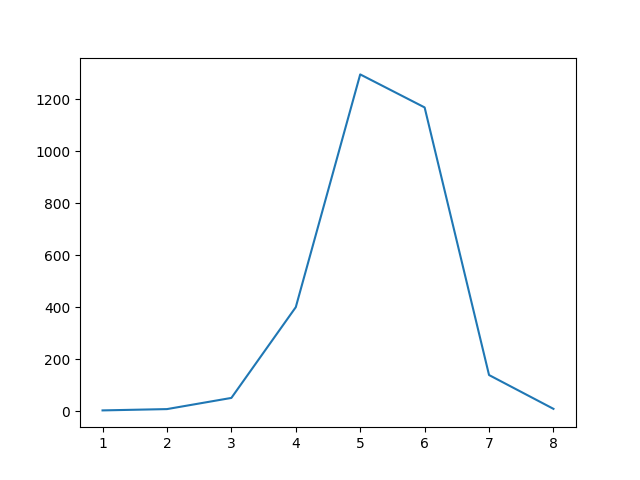
\includegraphics[width=1\textwidth]{img/categories_levels.png}
	\caption{Wykres przedstawiający liczby kategorii na poszczególnych poziomach drzewa.}
	%\label{fig:warstwy}
\end{figure}
Najwięcej artykułów z kolei jest przypisanych do kategorii z poziomów 4 i 5, średnio artykuł jest przypisany do kategorii z poziomu 4,63. Średnio na kategorię będącą liściem w drzewie przypada 7,71 artykułu.
\begin{figure}[H]
	\centering
	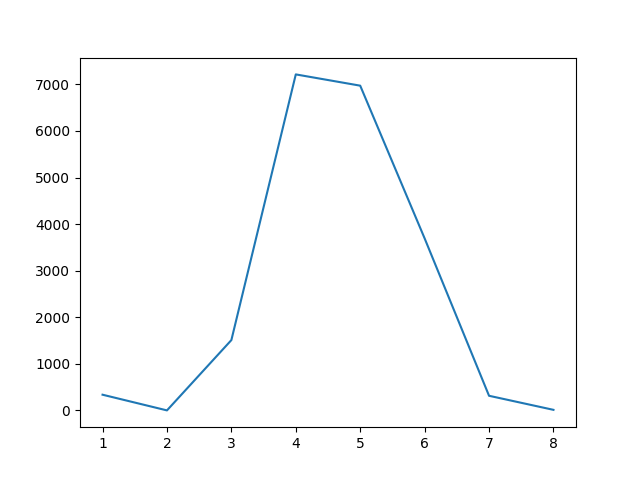
\includegraphics[width=1\textwidth]{img/cat_art_levels.png}
	\caption{Wykres przedstawiający liczby artykułów, dla których kategoria na danym poziome drzewa jest tą najbardziej szczegółową.}
	%\label{fig:warstwy}
\end{figure}
Po wstępnej analizie system kategorii oceniam jako spójny i rzetelny. Uważam, że można użyć go jako punkt odniesienia przy konstrukcji metod ewaluacji testowanych technik określania podobieństwa między artykułami.
\subsection{Słowa kluczowe}
Do każdego artykułu dołączona jest lista słów kluczowych. Są to wyrażenia złożone z jednego lub kilku słów, które mają za zadanie scharakteryzować w skrócie jego zawartość, np.~,,aparaty'', ,,aparaty cyfrowe'', ,,lustrzanki'', ,,Sony''. Pole to jest wykorzystywane w dotychczasowym mechanizmie generowania rekomendacji - artykuły podobne do danego są wyszukiwane na podstawie jego słów kluczowych. Przyglądając się wszystkim słowom kluczowym zestawionym razem zauważyłem pewne niespójności: część słów kluczowych o tej samej treści pisana jest w inny sposób, np.~różną wielkością liter, czy używając myślnika zamiast spacji. Wynika to zapewne z faktu przypisywania słów kluczowych samodzielnie przez autorów w oderwaniu od słów przypisanych do reszty artykułów. Średnio każdy artykuł ma przypisane 5,8 słów kluczowych, natomiast unikalnych słów kluczowych w skali całego korpusu jest 60403.

\section{Wstępne przetwarzanie danych}

W celu zwiększenia skuteczności metod analizy tekstu stosuje się wstępne przetwarzanie danych. Ma ono na celu takie przygotowanie tekstu, aby zmaksymalizować jakość wyników operujących na nim później algorytmów. Techniki wstępnego przetwarzania tekstu nie wchodzą w skłąd żadnego standardu - dobieram je indywidualnie do konkrtenego przypadku, zgodnie z intuicją.

Niżej opisuję kolejne kroki wstępnego przetwarzania tekstu, które wykonuję na posiadanym zbiorze artykułów.
\begin{enumerate}
	\item Oczyszczanie tekstu ze zbędnych, wspomnianych wcześniej znaczników. Z punktu widzenia semantycznej analizy tekstu są one bezużyteczne, czy wręcz szkodliwe (powodują pewne ,,zanieczyszczenie'' tekstu). Stąd usuwam je wykorzystując odpowiednio skonstruowane wyrażenia regularne.
	\item Usunięcie ,,słów stopu''(ang. stopwords) - na ogół krótkich słów nie wnoszących nic do znaczenia całości artykułu. Są to np.~,,w'', ,,z'', ,,ponieważ''. Ich usunięcie zmniejsza liczbę słów dokumentu skracając tym samym czas jego przetwarzania. Jako że słowa te występują często, usunięcie ich daje możliwość uwypuklenia znaczenia innych słów mających wpływ na rzeczywiste znaczenie całego artykułu. Zbiór słów stopu czerpię z \cite{stopwords}.
	\item Sprowadzenie wszystkich słów dokumentu do małych liter. Pomaga to ujednolicić postać części słów o tym samym znaczeniu, wśród których jedno występuje na początku zdania a inne w środku.
	\item Rozbicie słów połączonych myślnikiem. Doświadczenie w późniejszym etapie (tokenizacji) pokazuje, że narzędzie jej dokonujące (Morfologik\cite{morfologik}) nie radzi sobie z tego typu słowami (np.~,,biało-czerwony'') i zostania je w niezmienionej postaci gramatycznej (np.~,,biało-czerwonego''). Stąd konieczność ręcznego wykonania przeze mnie mechanizmu rozbijającego takie słowa do postaci kompatybilnej z tokenizerem. Do wykonania odpowiedniej funkcji potrzebna była wcześniejsza analiza tego typu słów pod kątem zachowania obu członów w zależności od ich rodzaju, przypadku i występowania konkretnych liter w sufiksach słów składowych. Zależało mi także, aby nie rozbijać słów będących nazwami własnymi, czy symbolami urządzeń.
	\item Tokenizacja. Jest to najistotniejszy element całego procesu. Polega na sprowadzaniu słów o tym samym znaczeniu, a różnej formie gramatycznej do tej samej postaci. Sporym utrudnieniem jest tutaj stopień skomplikowania języka polskiego oraz liczba wyjątków, jaką ten język posiada. Za przykład może posłużyć słowo ,,mieć'', którego jedna z form to ,,ma'', kolejna to ,,miej''. Celem etapu jest sprowadzenie każdego z tych wyrazów do formy podstawowej ,,mieć''. Do przeprowadzenia tej operacji stosuję narzędzie Morfologik\cite{morfologik}.
\end{enumerate}

Użycie wymienionych technik nie jest jedynym standardem a wynikiem analizy przetwarzanych danych i techniki te zostały dobrane dla tego konkretnego przypadku

\section{Opis danych po wstępnym przetwarzaniu}

Powyższe kroki doprowadzają dane do stanu, w którym można zastosować techniki semantycznej analizy tekstu. Słownik zbudowany na wstępnie przetworzonym korpusie zawiera 98174 unikalnych słów, oraz 7409145 wszystkich słów (z powtórzeniami).

\begin{figure}[H]
	\centering
	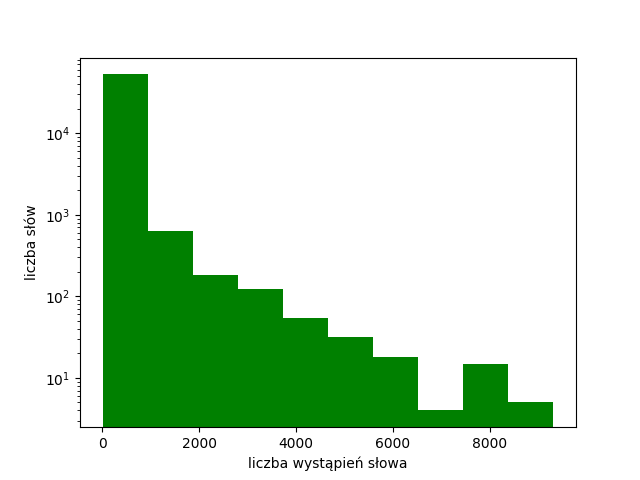
\includegraphics[width=1\textwidth]{img/words_hist_log.png}
	\caption{Histogram liczby wystąpień słów w korpusie w skali logarytmicznej.}
	%\label{fig:warstwy}
\end{figure}

Większość artykułów okazała się być podobnej długości, średnia długość artykułu to 370 słów.

\begin{figure}[H]
	\centering
	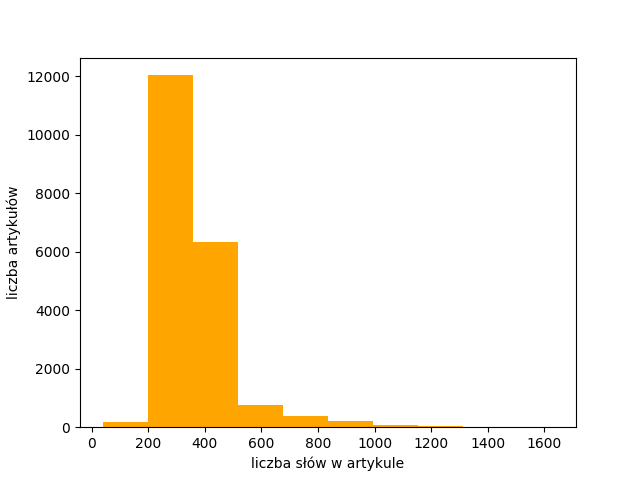
\includegraphics[width=1\textwidth]{img/articles_length_hist.png}
	\caption{Histogram długości artykułów.}
	%\label{fig:warstwy}
\end{figure}

\chapter{Metody ewaluacji}

W celu porównania stosowanych metod wyznaczania podobieństwa między artykułami konieczna jest formalizacja pewnych miar tego podobieństwa. W opisie znanych ogólnych miar posłużyłem się pojęciem ,,relewantności'' --- formalną wartością wyrażoną za pomocą liczb rzeczywistych. Jednakże w praktyce rzadko dysponuje się wartością, na ile dany element rankingu jest adekwatny do zapytania, generującego ów ranking.  

Ewaluacja rankingu, w którym trafność wyników zależy od zachowania realnych użytkowników jest zadaniem nietrywialnym. Podobieństwo artykułów napisanych w języku naturalnym jest rzeczą subiektywną. W sytuacji idealnej dysponowałbym obiektywną miarą podobieństwa pomiędzy parami $N$ artykułów (np.~wyznaczoną wcześniej przez miarodajną grupę użytkowników), które to $N$ artykułów stanowiłoby zbiór testowy. Uzyskanie takich danych wiąże się jednak z dużymi kosztami i leży poza moimi możliwościami.

Inną praktyką umożliwiającą obiektywną ocenę, wykorzystywaną w działających systemach są tzw. testy A/B polegające na podziale użytkowników na grupy i zaaplikowaniu każdej grupie innego rozwiązania. Następnie mierzone są pewne wskaźniki wśród każdej grupy (w naszym przypadku np.~liczba ,,kliknięć'' prawdziwych użytkowników w artykuły rekomendowane) i spośród zgromadzonych wyników wybierane jest rozwiązanie najlepsze.

Z powodu braku możliwości wykorzystania do ewaluacji rozwiązań rzeczywistych użytkowników serwisu internetowego jestem zmuszony wprowadzić własne miary oparte na dostępnych danych. Należy tu zaznaczyć niedoskonałość wprowadzanych miar, ponieważ każda z nich opiera się na pewnych założeniach, od których prawdziwości zlaeży jakość całej miary.

Testowane metody adaptuję tak, aby na podstawie pewnego artykułu bazowego otrzymywać listę artykułów podobnych do niego uszeregowanych pod kątem relewantności malejąco. Takie działanie można sformalizować w postaci funkcji $S_p: a_j \to \{a_{i}\}_{i < p}$, gdzie $a$ to artykuł, a $p$ to liczba elementów zwracanego ciągu. Funkcja $S$ przyjmuje artykuł tekstowy i zwraca skończony ciąg artykłów do niego podobnych zgodnie ze stopniem dopasowania (najlepsze na początku). Celem działania niżej opisanych miar jest każdej parze postaci: artykuł wejściowy-jeden z wyznaczonych artykułów podobnych przypisać ocenę tego podobieństwa --- relewantność. Np. metoda $S$ dla artykułu $X$ zwraca ciąg {$Y_1$, $Y_2$, ...}. Dla każdej z par za pomocą poniższych metod ewaluacji można określić relewantność np.~$rel(X, Y_1) = a_1, rel(X, Y_2) = a_2$ itd. Następnie wyniki dla metody $S$ i wejścia $X$ należy zagregować. Dokonuję tego na dwa sposoby.
\begin{itemize}
	\item Obliczenie średniej $\frac{1}{p}\sum_{i=1}^{p}relevance(X,Y_1)$.
	\item Użycie metody nDCG, gdzie relewantność to wynik poszczególnych ewaluacji podobieństwa artykułów.
\end{itemize}  


Oceny dla konkretnej metody, dla ustalonej próby par artykułów są następnie wykorzystane do wyznaczenia wartości średniej  miary nDCG tej metody.


\section{Miara 1: Dystans oparty na metadanych}

Jak wspomniałem wcześniej dane prócz treści artykułów zawierają również pewne metadane, a wśród nich umożliwiające tworzenie powiązań między artykułami. Skupiam się tu na polach: ,,słowa kluczowe'' i ,,kategoria''.

\subsection{Kategorie} 

Pierwszą zastosowaną miarą, pozwalającą ocenić jakość dopasowania podobnych artykułów jest ich odległość we wcześniej wspomnianym drzewie kategorii. Formalnie wartość miary to długość części wspólnej ścieżek od korzenia drzewa kategorii do węzłów reprezentujących artykuły. Im więcej wspólnych przodków w drzewie, tym bardziej podobne do siebie są artykuły reprezentowane przez węzły drzewa. Zaletą miary jest fakt, iż przypisanie artykułu do kategorii zostało wykonane przez autora, którego można określić ekspertem w dziedzinie tematyki artykułu. Stąd przynależność artykułu do danej kategorii jest mocno uzasadniona. Kolejną zaletą tej miary jest fakt, iż można ją zastosować automatycznie - wiedza ekspercka jest już zapisana w metadanych artykułów. Należy zaznaczyć tu jednak, że miara nie jest idealna - każdy artykuł należy do tylko jednego liścia drzewa kategorii. Stąd artykuł poruszający zagadnienia z różnych obszarów, który można by przypisać dwóm stosunkowo odległym kategoriom $A$ i $B$, zostanie przypisany tylko do jednej kategorii, np.~$A$. Miara pokaże wtedy dużą odległość od artykułów z kategorii $B$, co nie jest prawdą.

Za przykład mogą posłużyć drzewa na poniższych rysunkach. W drzewie 1. artykuły $X$ i $Y$ mają dwie wspólne kategorie, stąd $relevance(X, Y) = 2$. Natomiast artykuły $Y$ i $Z$ z drugiego drzewa mają trzech wspólnych przodków, stąd $relevance(Y, Z)=3$ Miara wskazuje, że artykuły $X$ i $Y$ są do siebie mniej podobne, niż artykuły $Y$ i $Z$.

\begin{figure}[H]
	\centering
	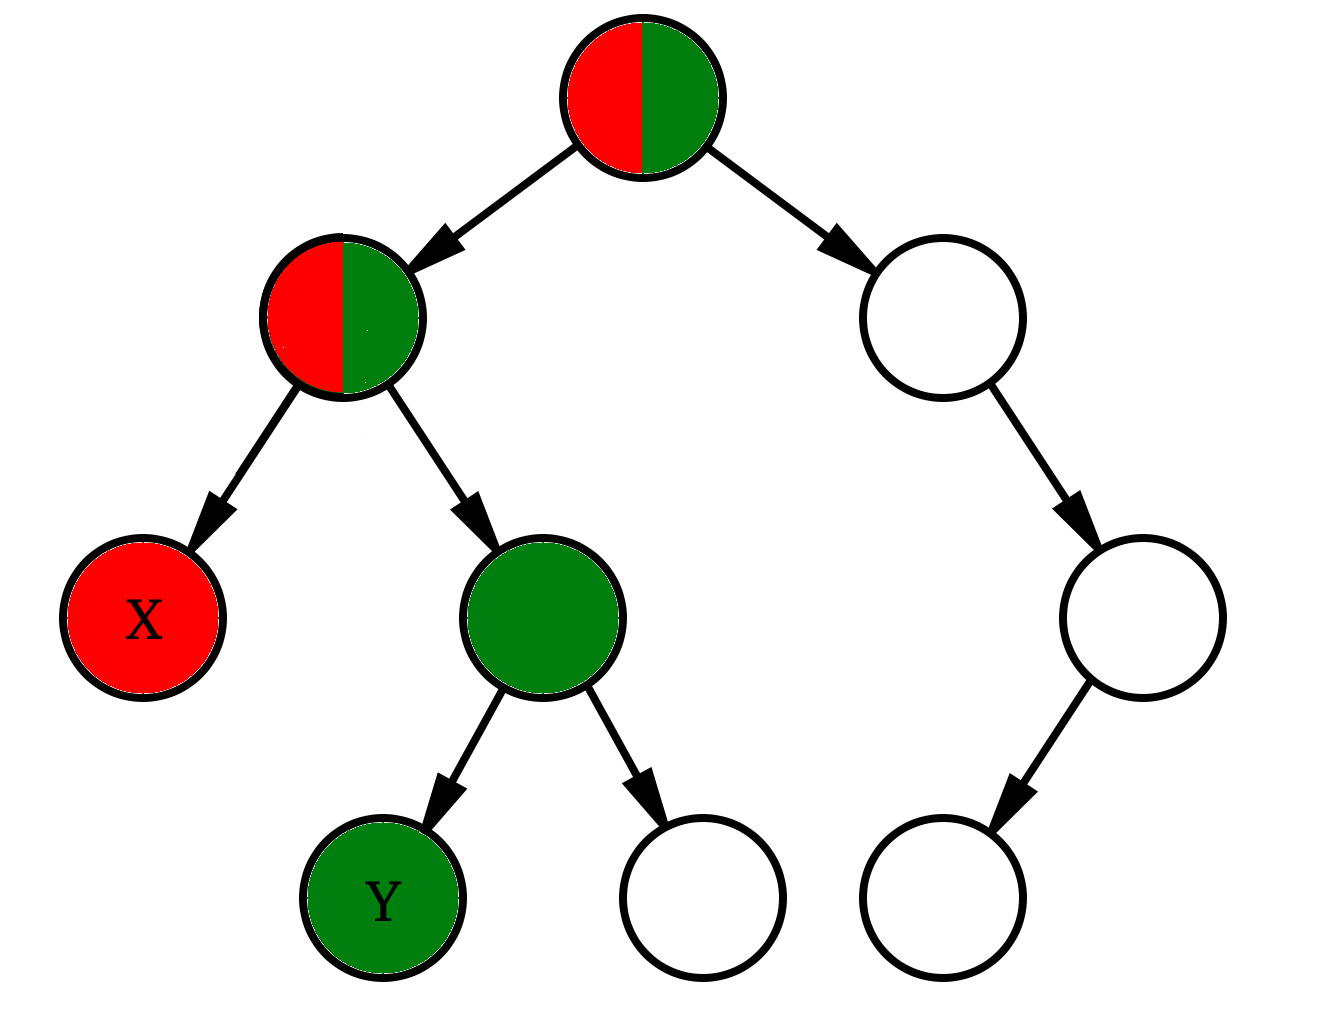
\includegraphics[width=0.5\textwidth]{img/cat_tree_example_1.png}
	\caption{Drzewo kategorii dla przykładu 1.}
	%\label{fig:warstwy}
\end{figure}
\begin{figure}[H]
	\centering
	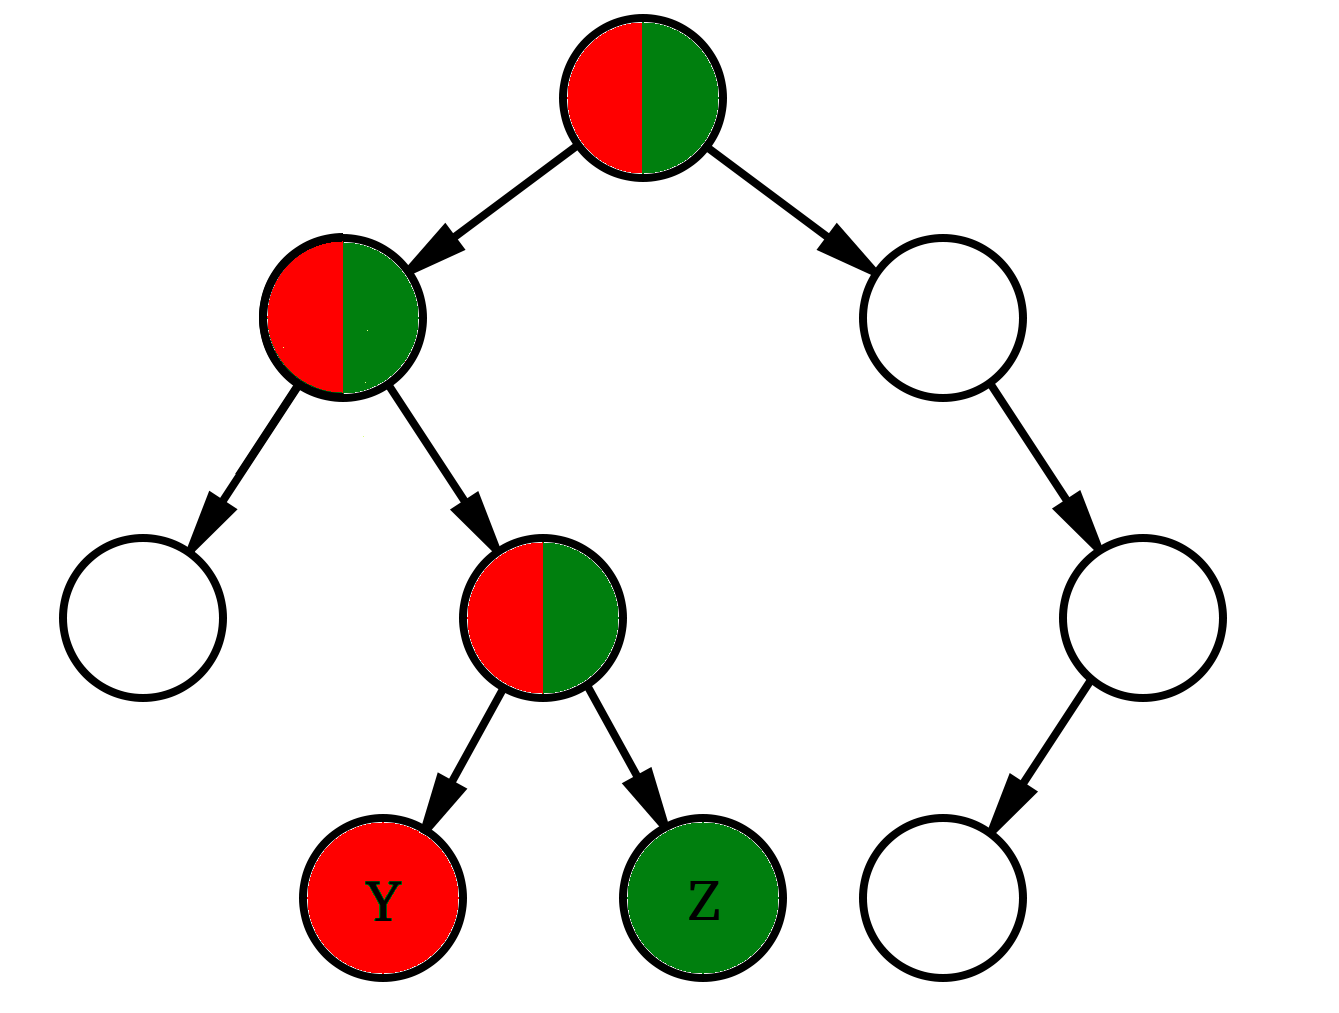
\includegraphics[width=0.5\textwidth]{img/cat_tree_example_2.png}
	\caption{Drzewo kategorii dla przykładu 2.}
	\label{fig:warstwy}
\end{figure}


\subsection{Słowa kluczowe}

Kolejna miara oparta na metadanych artykułów korzysta ze słów kluczowych. Wśród ogółu słow kluczowych występują niespójności, których większość zlikwidowałem poprzez sprowadzenie słów od małych liter oraz usunięciu ,,słów stopu''. Po tej unifikacji liczba unikalnych słów kluczowych to 58565.

Niniejsza miara działa podobnie do poprzedniej opartej o kategorie. Para artykułów otrzymuje 1 punkt za każdą wspólną parę posiadanych kategorii. Np. dla artykułu $X$ o słowach kluczowych \{,,$kosmetyki$'', ,,$kremy$'', ,,$zmarszczki$''\} oraz $Y$ o słowach kluczowych \{,,$kosmetyki$'', ,,$zele do wlosow$'', ,,$kremy$'', ,,$szampony$''\} $relevance(X,Y)=2$, ponieważ oba artykuły mają dwa wspólne słowa kluczowe ($,,kosmetyki''$ i $,,kremy''$).

\section{Miara 2: Historyczna aktywność użytkowników serwisu}

Zbieranie a następnie przechowywanie informacji o aktywności użytkownika w ramach serwisu internetowego jest powszechną praktyką. Proces ten pozwala na analizę zachowania użytkowników co może doprowadzić do wniosków, jakie usprawnienia należy przedsięwziąć, aby spełnić cele biznesowe. Jednym z przykładów aktywności użytkownika zapisywanej przez serwis Allegro są kliknięcia w linki znajdujące się na stronie internetowej. Informacja ta pozwala sporządzić jeszcze jedną miarę jakości dopasowania podobnych do siebie artykułów. Postać danych, jakie udało mi się uzyskać z serwisu to tabela o polach: adres strony, na której nastąpiło kliknięcie, adres strony, na którą prowadzi link, data kliknięcia.

Jak już zostało opisane powyżej strona z artykułem tekstowym zawiera odnośiki do innych artykułów poruszających tematykę podobną do danego. Skoro zapisywana jest informacja o przejściach pomiędzy podstronami serwisu, to można obliczyć ile razy z artykułu $X$ dokonano przejścia na rekomendowany do niego artykuł $Y_1$, a ile razy na rekomendowany artykuł $Y_2$. Jeżeli liczba przejść na artykuł $Y_1$ jest większa niż na $Y_2$, można wnioskować, iż $Y_1$ wydaje się być bardziej relewantną rekomendacją dla artykułu $X$.

Posługując się powyższym założeniem, można zaproponować miarę jakości rekomendacji generowanych przez testowane metody w odniesieniu do popularności rzeczywistych rekomendacji wyekstrahowanej z danych serwisu o aktywności użytkowników.

W tym celu dokonuję adaptacji miary nDCG. Załóżmy, że testowana metoda $A$ zwraca pewien ciąg $p$ artykułów $c_A=a_1,\ a_2,\ ...,\ a_p$ podobnych do danego artykułu $x$, w kolejności od najbardziej relewantnego. Załóżmy również, część elementów ciągu $c_B$ artykułów rekomandowanych w serwisie dla $x$ (używaną dotychczas w serwisie metodą $B$) znajduje się również w ciągu $c_A$, tj. $(\exists{a_i, a_j\in c_A})a_i \in c_B \land a_j \in c_B$, gdzie $i$, $j$ to indeksy w ciągu $c_A$. Załóżmy ponadto, że z danych o kliknięciach użytkowników w linki w ramach serwisu wiadomo, że przejście z $x$ na $a_i$ jest bardziej popularne niż przejście z $x$ na $a_j$. Stąd jeżeli $i<j$ ($i>j$), to jakość działania metody $A$ jest dobra (zła), bo metoda ta generuje podobne artykuły w kolejności zgodnej ze stopniem podobieństwa z artykułem bazowym, opartym o częstośc przejść użytkowników między artykułami.

Za miarę relewantności używaną przez nDCG przyjmuję liczby rzeczywistych przejść pomiędzy artykułami, a samą metodę stosuję tylko do przecięcia zbioru artykułów podobnych do danego generowanych przez daną metodę ze zborem artykułów rekomendowanych do danego przez dotychczasową metodę działającą w serwisie.

Zaletą metody jest, iż można ją zastosować automatycznie, lecz jest zależna od danych analitycznych pochodzących z serwisu, które są niedoskonałe.

\section{Miara 3: Ocena przez użytkowników offline}

Ostatnią opracowaną przez mnie miarą jest subiektywna ocena ekspercka. W celu obiektywizacji oceny, ewaluacja powinna być dokonana przez reprezentatywną grupę $T$ osób operujących na na tych samych danych. W metodzie tej grupa użytkowników dokonuje oceny podobieństwa par artykułów generowanych przez poszczególne testowane metody genreowania rekomendacji.

\begin{enumerate}
	\item Wybieram $n$ losowych artykułów bazowych $b_j, j=1,...,n$.
	\item  Testowaną metodą $M$ generuję $p$ artykułów $s_{jk}, k=1,...,p$ podobnych do każdego $b_j$ z $n$ wcześniej wylosowanych.
	\item Grupuję artykuły w pary: artykuł bazowy $b_j$ --- artykuł podobny $s_{jk}$.
	\item Za pomocą stworzonego interfejsu prezentuję każdemu z użytkowników kolejno wygerenowane pary w postaci rzeczywistych stron z artykułami dostępnych przez przeglądarkę internetową. Co ważne każdy użytkownik otrzymuje ten sam zestaw par. Podczas prezentacji pary użytkownik za pomocą interfejsu webowego ocenia podobieństwo pomiędzy artykułami $rel(b_j, s_{jk})$ w skali 1-10.
	\item Dla każdej pary obliczam średnią ocen wszystkich $T$ użytkowników $avg(j,k)=\frac{1}{T}\sum_{t}^{T}rel_t(b_j, s_{jk})$, gdzie $rel_t$ to ocena $t$-go użytkownika.
	\item Dla każdego artykułu bazowego $b_j$ obliczam $m(j) = \frac{1}{\sum_{i=1}^{p}i}\sum_{i=0}^{k} avg(j,k)*(p-i)$ będące średnią ważoną ocen, gdzie każdy kolejny artykuł podobny otrzymuje coraz mniejszą wagę.
	\item Oceną testowanej metody jest średnia $\frac{1}{n}\sum_{j}m(j)$.
\end{enumerate}

Wadą tej metody jest jej powolność i potrzeba zaangażowania dodatkowych osób dokonujących ewaluacji. Niemożliwym wydaje się przeprowadzenie badania dla wszystkich artykułów, stąd konieczny jest wybór losowej próby artykułów, które parami poddane zostaną ocenie pod kątem podobieństwa.


\chapter{Opis testów}

W przeprowadzanych testach staram się dokonać porównania pomiędzy różnymi konfiguracjami tej samej metody oraz pomiędzy najlepszymi wariantami różnych metod. W tym celu wykorzystuję wprowadzone miary ewaluacji. W większości przypadków używam miar automatycznych bazujących na metadanych artykułów oraz historycznej aktywności użytkowników serwisu. Do ostatecznego porównania pomiędzy najlepszymi wariantami testowanych metod stosuję również miarę opartą na ocenie eksperckiej. Miara ta daje najbardziej rzetelne wyniki, jednakże jej użycie jest wyjątkowo kosztowne - wymaga zaangażowania osób testujących oraz sporych nakładów czasowych. Stąd zdecydowałem na użycie jej tylko w jednym przypadku.

\section{Testowane metody generowania rekomendacji}

Wykonuję szereg testów adaptacji metod semantycznej analizy języka naturalnego o różnych nazwach, w różnych konfiguracjach. Stąd dla czytelności wprowadzam niekiedy w nawiasach skrócone sygnatury tych metod, które stosuję w dalszej części pracy zamiast pełnych opisów.

\subsection{Metody oparte o modelowanie tematu}

Najważniejszym hiperparametrem metod tej grupy: LSI oraz LDA jest liczba tematów, stąd dokonuję testu jak zmiana tego parametru wpływa na jakość modelu.

\subsection{Metody oparte o word embedding}
Wykonuję testy adaptacji metod wektorowej reprezentacji słów dla wielu konfiguracji. Poniżej obszary, na których dokonuję zmian konfiguracji.

\subsubsection{Korpus bazowy}

Pierwszy model Word2vec, z jakim miałem styczność to model\cite{pias} stworzony m.in. przez dr inż. M. Piaseckiego z Politechniki Wrocławskiej dostępny poprzez stronę internetową. Model ten był uczony na korpusie Słowosieci wer. 10\cite{wordnet}. Zgodnie z opisem autorów dane przed uczeniem  przeszły segmentację, lematyzację i ujednoznacznianie morfosyntaktyczne. Użyte parametry uczenia Word2Vec: metoda skip gram, wekroty długości 100, okno kontekstu wielkości 5.

Model ten zawiera 73875 spośród 98174 (75\%) unikalnych słów korpusu artykułów Allegro oraz 7313915 z 7409145 (99\%) wszystkich słów korpusu artykułów. Wskazuje to, iż słowa nieobecne w modelu są bardzo mało popularne w korpusie artykułów (stanowią ok 1\% całości). Po samodzielnym sprawdzeniu stwierdzam, że słowa nieobecne w modelu to: ,,literówki'' lub słowa niepoprawnie stokenizowane (np. ,,urządzeia''), symbole marek produktów (np.~,,ux305fa'', ,,i7-4700qm''), żargon branżowy (np.~,,bootsów''), złożenia wyrazów (np.~,,kurzoodporne''), wyrazy obce lub ich spolszczenia (np.~,,thermoprotect''). Uważam, iż mimo niewielkiej liczby tych słów w stosunku mogą mieć one znaczący wpływ na semantykę artykułów.

W związku z powyższym stwierdzeniem wykonuję naukę modelu Word2vec również na własnym korpusie artykułów w celu zawarcia brakujących w poprzednim modelu słów. Najrozsądniejszym postępowaniem byłoby tutaj rozszerzenie modelu opartego na korpusie Słowosieci również o brakujące słowa, jednak metoda Word2vec nie pozwala na dodanie nowych słów do słownika istniejącego modelu, a jedynie na dalszą naukę w oparciu o słowa już istniejące w słowniku. Siłą rzeczy model zbudowany na zbiorze artykułów zawiera wszystkie słowa występujące w artykułach słowa. Korpusu tego używam do tworzenia modelów w oparciu o wszystkie pozostałe sposoby.

Dokonuję porównania jakości modelu uczonego na korpusie Słowosieci z modelem uczonym na korpusie artykułów Allegro.

\subsubsection{Sposób generowania wektorów i długość wektorów}
Do wygenerowania wektorów reprezentujących słowa używam metod wektorowej reprezentacji tekstu: Word2vec, GloVe oraz FastText. Każdą z nich testuję pod kątem różnej wymiarowości generowanych wektorów.

\subsubsection{Metoda określenia podobieństwa między wektorowymi reprezentacjami dokumentów}
Zadaiem metod ,,word embedding'' jest wygenerowanie wektorowej reprezentacji słowa. W celu porównania całych dokumentów i wyznaczenia podobieństw między nimi należy użyć dodatkowych środków. W tym celu korzystam z poniższych metod:
\begin{enumerate}
	\item odległość cosinusowa pomiędzy centroidami wektorowej reprezentacji tekstów (w skrócie metoda centroidu),
	\item Word Mover's Distance,
	\item autorska metoda wykorzystująca odległość cosinusową pomiędzy wektorową reprezentacją słów kluczowych wyznaczonych metodą LDA. Celem metody jest zmniejszenie wymiarowości artykułu oraz użycie tylko znaczących słów przy obliczaniu centroidu artykułu. W tej metodzie za pomocą LDA wyznaczam słowa kluczowe, które z największą wagą przynależą do danego artykułu. Nauczony model LDA każdemu dokumentowi $i$ przypisuje zestaw tematów z określonymi wagami przynależności $t_{ij}$ oraz każdemu tematowi $j$ przypisuje zestaw słów wraz z wagami $w_{jk}$. Na tej podstawie dla każdego artykułu $i$ mogę wybrać $p$ słów, które posiadają najwyższą wagę przynależności do artykułu liczoną wg. wzoru $x(i,k)=\sum{j}t{ij}*w{jk}$, gdzie $k$ to dane słowo. Ostatecznie artykuł reprezentuję jako centroid $n$ słów o najwyższym $x$ dla danego słowa. W dalszych testach przyjmuję $n$ jako 10.
\end{enumerate}

Powyższe metody stosuję w celu wyznaczenia dla danego artykułu $a$ $p$ artykułów najbardziej do niego podobnych uszeregowanych majeląco pod względem relewantności do artykułu bazowego $a$.

\subsection{Elasticsearch}
W celu porównania z metodami semantycznymi testuję również dotychczasowe zapytanie do silnika Elasticsearch używane dotychczas w Allegro. Zapytanie to odpowiada listą $p$ artykułów najbardziej zbliżonych do artykułu wejściowego w kolejności od najbardziej podobnego

\subsection{Metoda losowa}
W celu posiadania punktu odniesienia dokonuję testów dla metody losowo wybierającej $p$ podobnych do danego artykułów. Wybór następuje zgodnie z rozkładem jednostajnym ze zbioru wszystkich artykułów.

\section{Metody ewaluacji}

W celu wykonania oceny testowanych metod wykorzystuję wszystkie metody ewaluacji opisane w rozdziale 4, które opatruję skróconymi sygnaturami.
\begin{enumerate}
	\item $clicks$ - ocena na podstawie historycznej aktywności użytkowników mierzona na podstawie liczby kliknięć w odnośniki.
	\item $mut\_cat[\_ndcg]$ - relewantność wyszukanych artykułów liczona na podstawie liczby wspólnych kategorii z artykułm bazowym. Stosuję dwa warianty: średnia relewantność wyszukanych artykułów oraz miara nDCG.
	\item $mut\_kw[\_ndcg]$ - relewantność wyszukanych artykułów liczona na podstawie liczby wspólnych słów kluczowych z artykułm bazowym. Również stosuję dwa warianty: średnia relewantność wyszukanych artykułów oraz miara nDCG.
	\item $users$ - ocena na podstawie eksperckiej oceny użytkowników. W badaniu wykorzystałem 5 użytkowników operujących każdy na tym samym zbiorze par testowych. Pary zostały wygenerowane (zgodnie z wcześniejszym opisem metody) na podstawie 50 artykułów bazowych wylosowanych spośród wszystkich artykułów udostępnionych mi przez Allegro.
\end{enumerate}





\chapter{Wyniki badań}
W rozdziale tym przedstawiam wyniki oceny jakości poszczególnych metod w zależności od ich hiperparametrów. Oceny dokonuję na podstawie opisanych uprzednio miar. Do wyników każdego testu dołączam ich interpretację oraz wnioski.

\subsection{LSI w zależności od liczby tematów}

Dokonuję porównania jakości modelu LSI w zależności od wartości hiperparametru - liczby tematów.

\begin{table}[H]
	\centering
	\begin{tabular}{lrrrr}
		\hline
		&       100 &      300 &      500 &      600 \\
		\hline
		mut\_cat      & 3.43131   & 3.50634  & 3.52346  & 3.51793  \\
		mut\_kw       & 1.77666   & 2.20166  & 2.38808  & 2.33861  \\
		mut\_cat\_ndcg & 0.507238  & 0.516217 & 0.518053 & 0.517515 \\
		mut\_kw\_ndcg  & 0.0972985 & 0.119504 & 0.129079 & 0.126829 \\
		clicks       & 0.865496  & 0.868586 & 0.878243 & 0.87366  \\
		\hline
	\end{tabular}
	\caption{Wyniki ewaluacji metody LSI dla zmiennej liczby tematów.}
\end{table}

\begin{figure}[H]
	\centering
	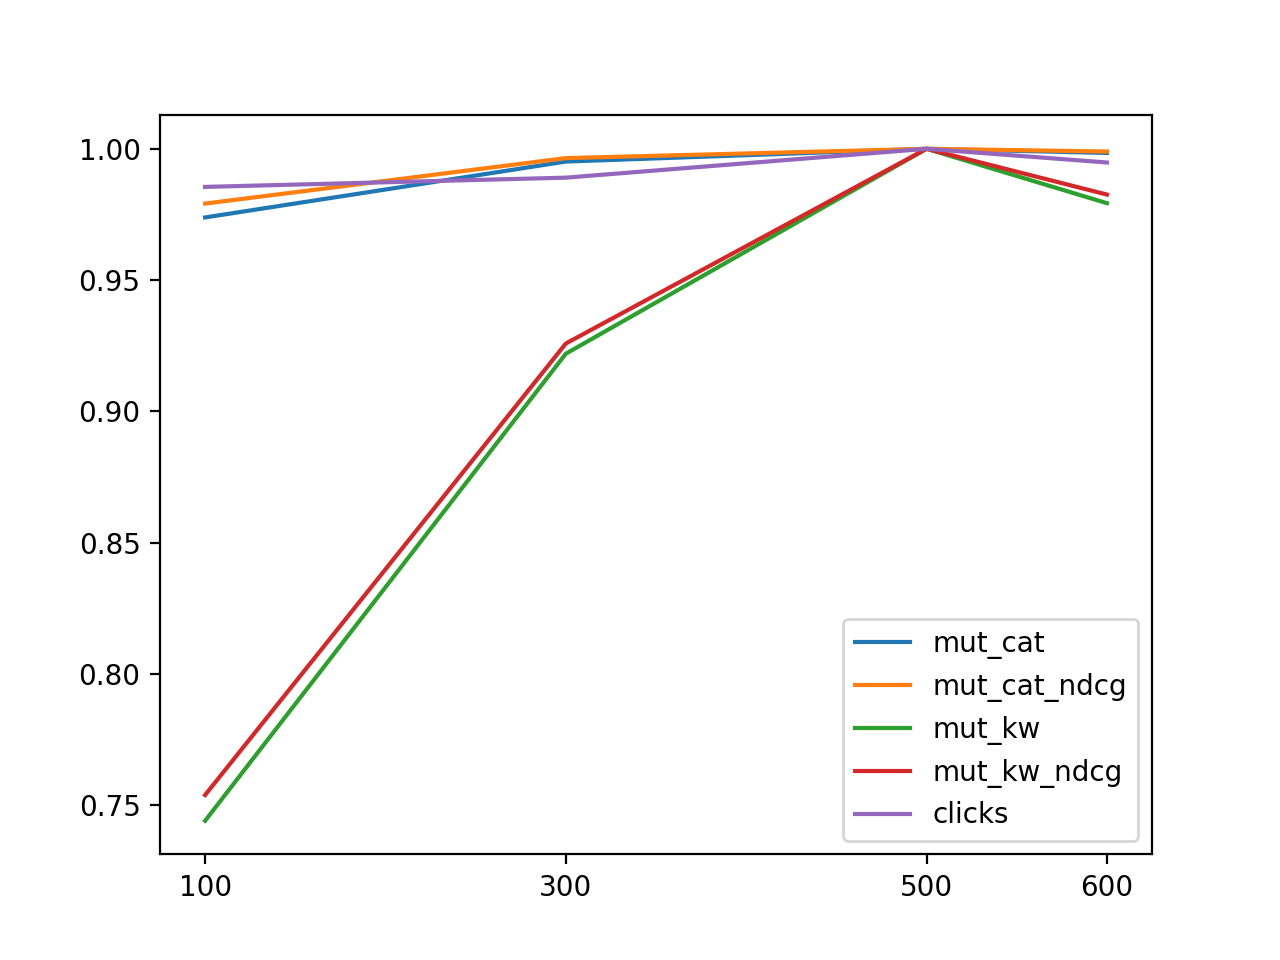
\includegraphics[width=1\textwidth]{img/results/lsi.png}
	\caption{Wykres porównujący znormalizowane wyniki dla metody LSI.}
	%\label{fig:warstwy}
\end{figure}

Miary oparte na liczbie wspólnych słów kluczowych ($mut\_kw...$) wyraźnie pokazują wzrost jakości modelu przy wzroście liczby tematów. Średnia wszystkich miar pokazuje, że najwyższą jakość model osiąga dla liczby tematów 500.

\subsection{LDA w zależności od liczby tematów}

Podobnie, jak w poprzednim punkcie dokonuję porównania jakości modelu LDA w zależności od wartości hiperparametru - liczby tematów.


\begin{table}[H]
	\centering
	\begin{tabular}{lrrrrrr}
		\hline
		&       100 &       300 &       500 &       700 &       900 &      1100 \\
		\hline
		mut\_cat      & 3.29108   & 3.34755   & 3.35077   & 3.36767   & 3.39972   & 3.3788    \\
		mut\_cat\_ndcg & 0.48793   & 0.495011  & 0.494236  & 0.497623  & 0.500823  & 0.498854  \\
		mut\_kw       & 1.31741   & 1.48792   & 1.58854   & 1.69146   & 1.76637   & 1.75904   \\
		mut\_kw\_ndcg  & 0.0733675 & 0.0815366 & 0.0880742 & 0.0919873 & 0.0961874 & 0.0963659 \\
		clicks       & 0.880891  & 0.90278   & 0.879733  & 0.906384  & 0.912387  & 0.890913  \\
		\hline
	\end{tabular}
	\caption{Wyniki ewaluacji metody LDA dla zmiennej liczby tematów.}
\end{table}

\begin{figure}[H]
	\centering
	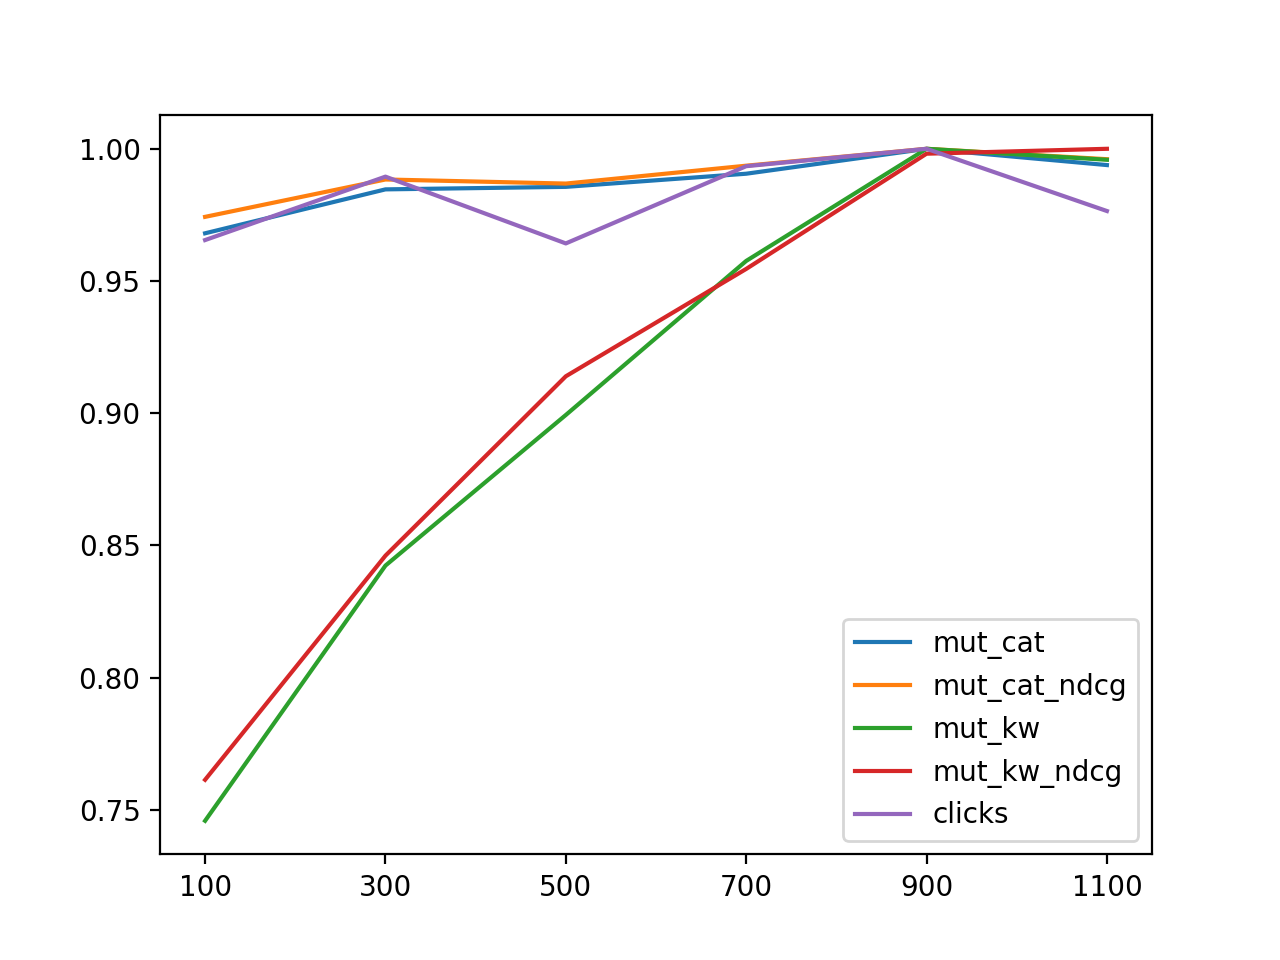
\includegraphics[width=1\textwidth]{img/results/lda.png}
	\caption{Wykres porównujący znormalizowane wyniki dla metody LDA.}
	%\label{fig:warstwy}
\end{figure}

Podobnie jak w przypadku modelu LSI miary oparte na liczbie wspólnych słów kluczowych ($mut_kw$) pokazują wzrost jakości modelu przy wzroście liczby tematów. Średnia wszystkich miar pokazuje, że najwyższą jakość model osiąga dla liczby tematów 900.


\section{Word2vec w zależności od korpusu}

Poniżej zestawiam wyniki dla modelów Word2vec o wektorach długości 100 uczonych: na korpusie artykułów z Allegro ($w2v100\_art$) oraz na korpusie Słowosieci ($w2v100\_wn$). Dokumenty porównywane są tu metodą centroidu.

\begin{table}[H]
	\centering
	\begin{tabular}{lrr}
		\hline
		&   w2v100\_art &   w2v100\_wn \\
		\hline
		mut\_cat      &    3.41328   &   3.38265   \\
		mut\_cat\_ndcg &    0.504018  &   0.496797  \\
		mut\_kw       &    1.66191   &   1.67062   \\
		mut\_kw\_ndcg  &    0.0896029 &   0.0885063 \\
		clicks       &    0.946487  &   0.946191  \\
		\hline
	\end{tabular}
	\caption{Wyniki ewaluacji metody Word2vec w zależności od korpusu, na którym trenowany był model.}
\end{table}

\begin{figure}[H]
	\centering
	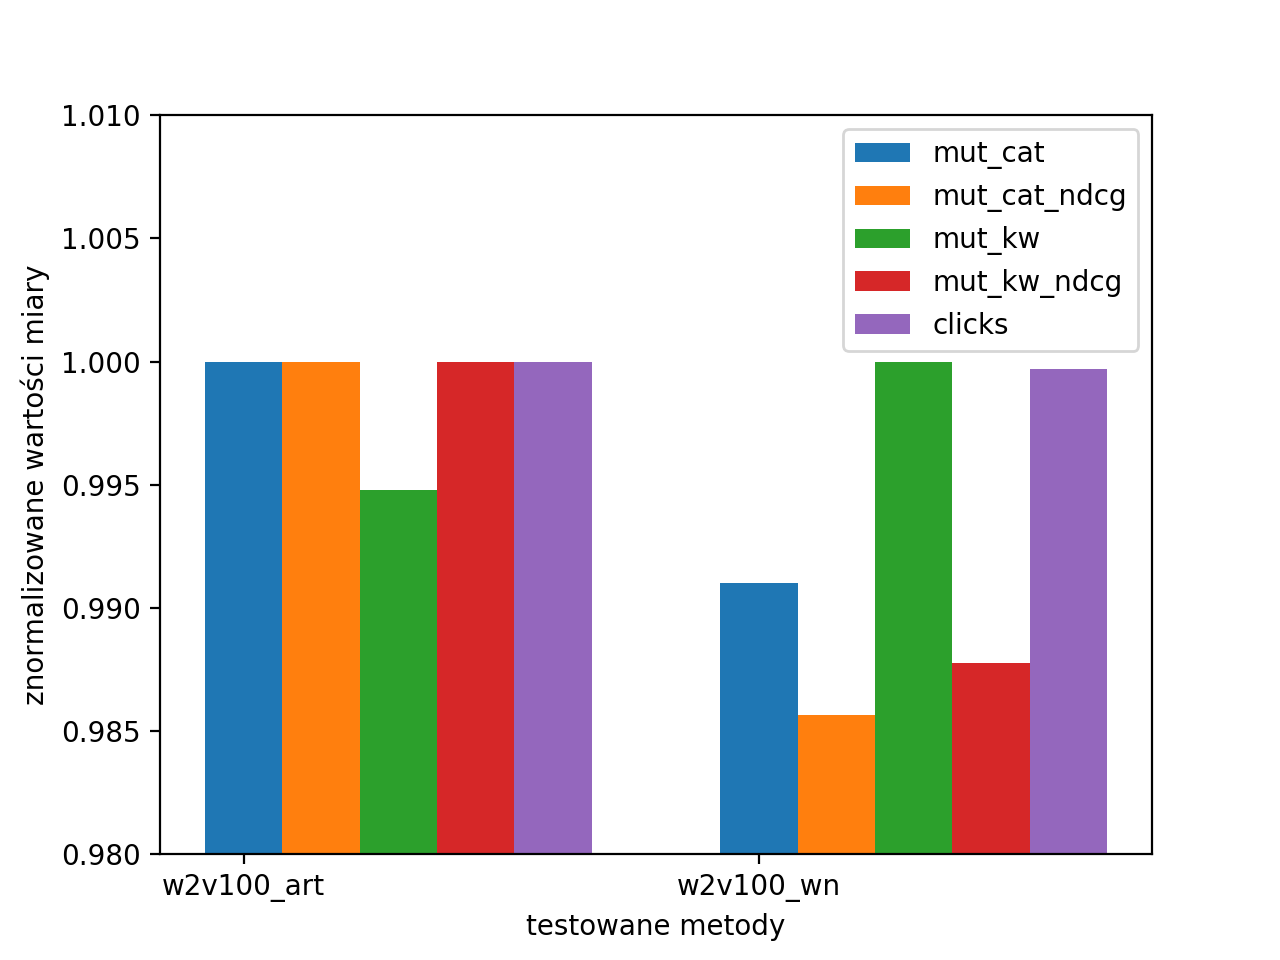
\includegraphics[width=1\textwidth]{img/results/w2v100_art_w2v100_wn_.png}
	\caption{Wykres porównujący znormalizowane wyniki dla metody Word2vec w zależnosci od bazowego korpusu.}
	%\label{fig:warstwy}
\end{figure}

Maksymalna różnica między najlepszym i najgorszym wynikiem nie przekracza 2\%. Stąd trudno jest stwierdzić, która metoda daje tu lepsze wyniki. Na korzyść modelu Word2vec uczonego na korpusie artykułów przemawia jego mały rozmiar, a co za tym idzie szybkość nauki. Z przyczyn braku wyraźnych zalet korzystania tu z modelu uczonego na korpusie słowosieci korzystam dalej jedynie z modeli opartych o korpus artykułów Allegro.

\section{Word2vec w zależności od metody porównywania dokumentów}

W niniejszym punkcie dokonuję porównania jakości metod określania podobieństwa między wektorowymi reprezentacjami dokumentów tekstowych wyznaczonymi metodą Word2vec dla wektorów długości 100 oraz 300. Biorę tu pod uwagę metody: centroidu całości dokumentu ($w2v100_centroid$), centroidu słów kluczowych wyznaczonych metodą LDA dla 100 tematów ($w2v100_lda100$) oraz Word Mover's Distance ($w2v100_wnd$). Z powodu powolności metody WMD stosuję ją do wyznaczenia dokumentów najbliższych danemu jedynie spośród 20 dokumentów najbardziej podobnych do danego wyznaczonych metodą centroidu.

\subsection{Wymiar wektorów: 100}

\begin{table}[H]
	\centering
	\begin{tabular}{lrrr}
		\hline
		&   w2v100\_centroid &   w2v100\_lda100 &   w2v100\_wmd \\
		\hline
		mut\_cat      &         3.41763   &       3.25386   &     3.17404  \\
		mut\_cat\_ndcg &         0.504596  &       0.482482  &     0.54389  \\
		mut\_kw       &         1.66962   &       1.2749    &     1.14807  \\
		mut\_kw\_ndcg  &         0.0900018 &       0.0701703 &     0.096873 \\
		clicks       &         0.938998  &       0.888249  &     0.996717 \\
		\hline
	\end{tabular}
	\caption{Wyniki ewaluacji metody Word2vec dla wektorów dł. 100 w zależności od metody porównywania wektorowych reprezentacji dokumentów.}
\end{table}

\begin{figure}[H]
	\centering
	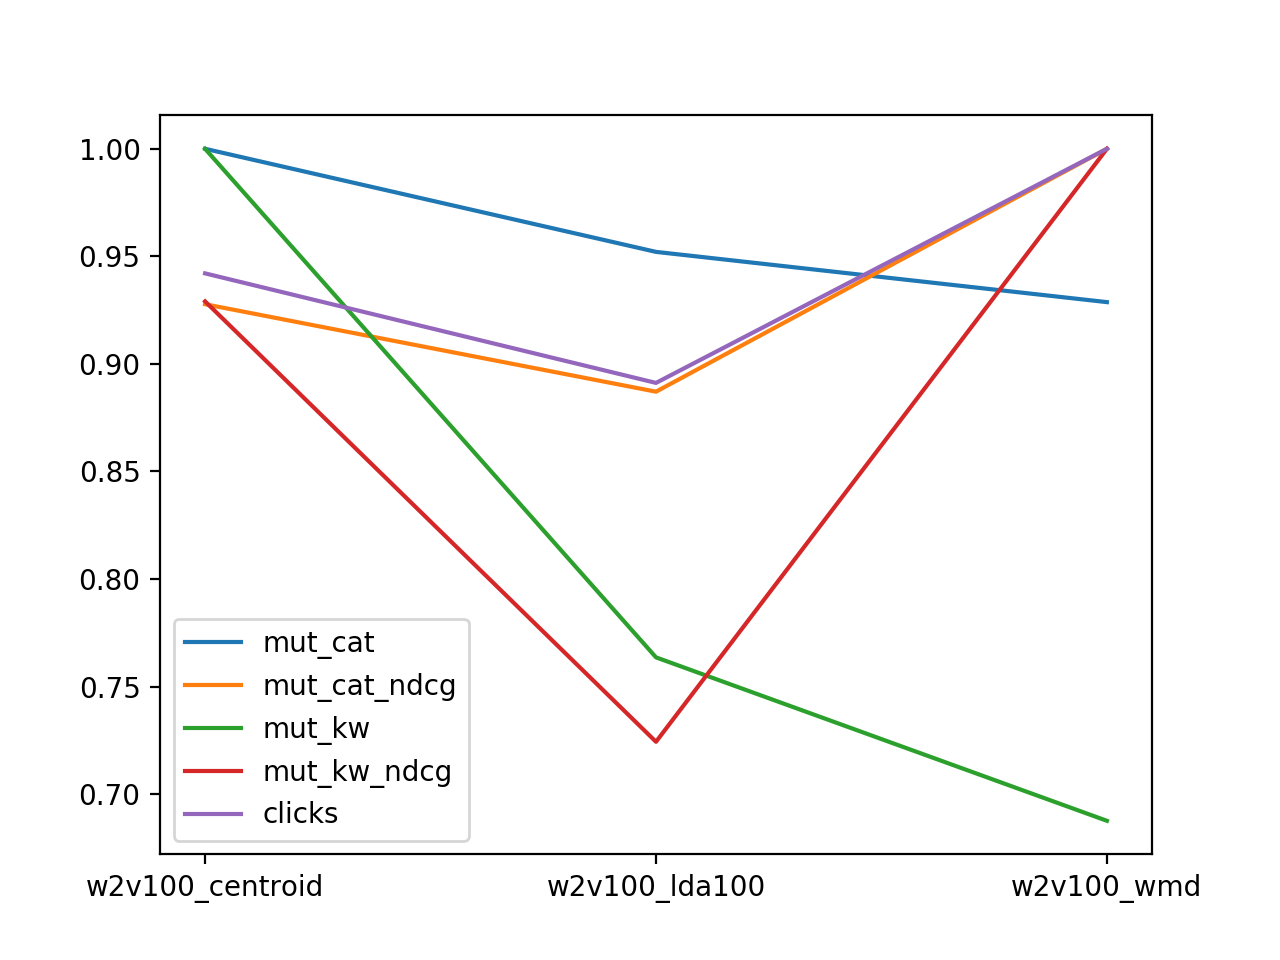
\includegraphics[width=1\textwidth]{img/results/w2v100_centroid_w2v100_lda100_w2v100_wmd_.png}
	\caption{Porównanie znormalizowanych wyników dla metody Word2vec w zależnosci od sposobu wyznaczania podobieństwa między wektorowymi reprezentacjami dokumentów.}
	%\label{fig:warstwy}
\end{figure}

\subsection{Wymiar wektorów: 300}


\begin{table}[H]
	\centering
	\begin{tabular}{lrrr}
		\hline
		&   w2v300\_ctr &   w2v300\_lda100 &   w2v300\_wmd \\
		\hline
		mut\_cat      &    3.42132   &       3.25724   &     3.1182   \\
		mut\_cat\_ndcg &    0.505457  &       0.482896  &     0.705453 \\
		mut\_kw       &    1.68395   &       1.27438   &     1.02838  \\
		mut\_kw\_ndcg  &    0.0906939 &       0.0701459 &     0.120046 \\
		clicks       &    0.936386  &       0.891596  &     0.940603 \\
		\hline
	\end{tabular}
	\caption{Wyniki ewaluacji metody Word2vec dla wektorów dł. 300 w zależności od metody porównywania wektorowych reprezentacji dokumentów.}
\end{table}

\begin{figure}[H]
	\centering
	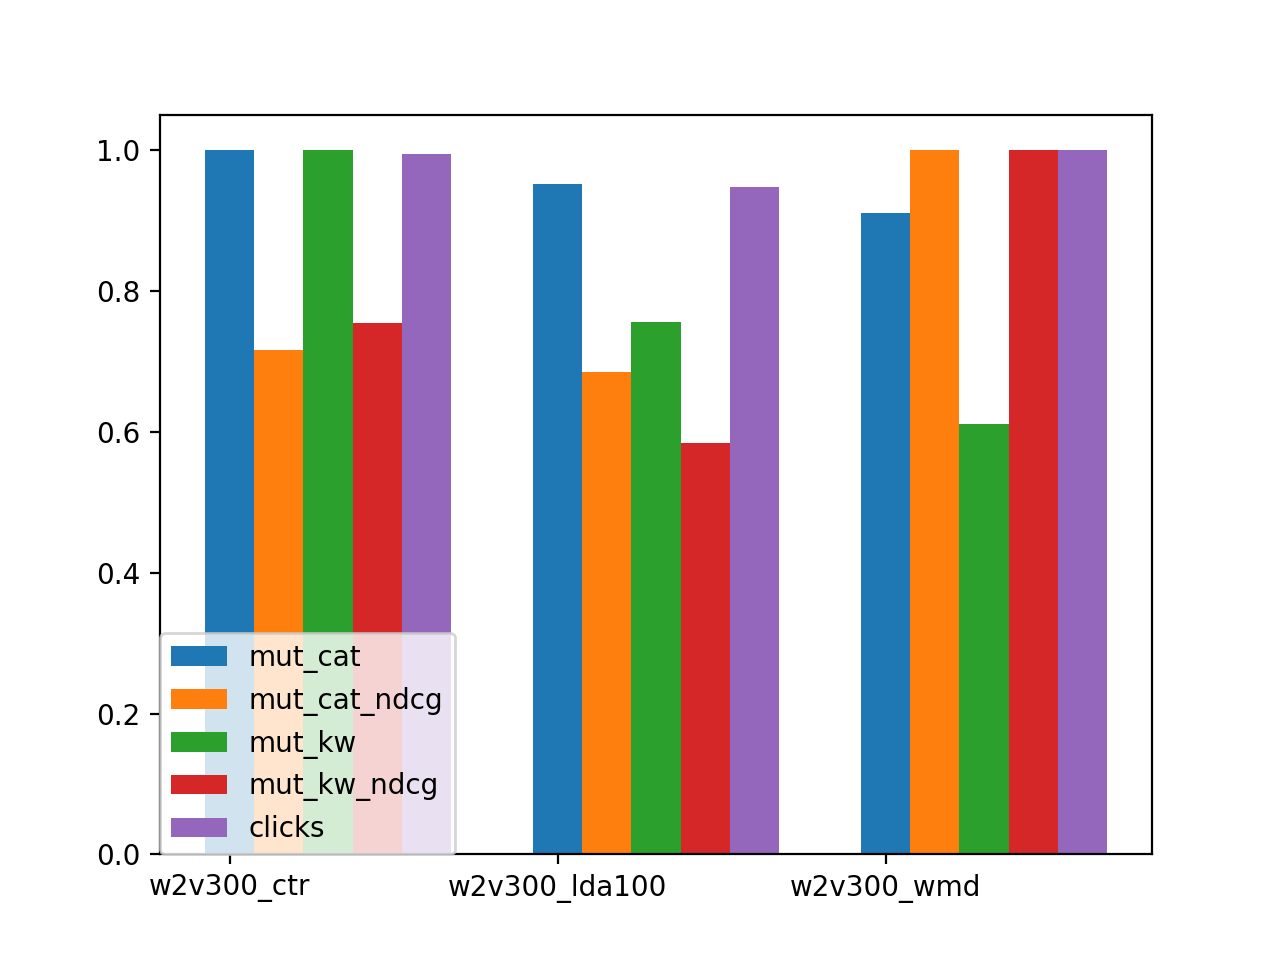
\includegraphics[width=1\textwidth]{img/results/w2v300_ctr_w2v300_lda100_w2v300_wmd_.png}
	\caption{Porównanie znormalizowanych wyników dla metody Word2vec w zależnosci od sposobu wyznaczania podobieństwa między wektorowymi reprezentacjami dokumentów.}
	%\label{fig:warstwy}
\end{figure}

Wyniki dla metody opartej o tematy LDA są jednoznacznie gorsze od wyników dla metody centroidu.

Dla obu konfiguracji metody Word2vec metoda Word Mover's Distance wykazuje się największą zdolnością do poprawnego szeregowania dokumentów (wysoki wskaźnik metod nDCG w porównaniu z metodami wykorzystującymi średnią).

Wadą metody WMD wykluczającą ją z użycia w tym przypadku jest jej powolność. Dla pierwszego przypadku  obliczenia trwały 55 minut, co przy czasie <1sek dla centroidu jest wartościa niedopuszczalną. Proporcjonalnie użycie tej metody dla całego korpusu trwałoby ok. 183 godzin.


\section{Metody word embedding w zależności od wymiarowości wektorów}

W niniejszym punkcie porównuję jakość metod word embedding (Word2vec, GloVe i FastText) w zależności od wymiarowości wektorów: 100, 300 i 1000. Użyta metoda wyznaczania podobieństwa dokumentów to metoda centroidu.

\subsection{Word2vec}

\begin{table}[H]
	\centering
	\begin{tabular}{lrrr}
		\hline
		&       100 &       300 &      1000 \\
		\hline
		mut\_cat      & 3.41328   & 3.42132   & 3.41763   \\
		mut\_cat\_ndcg & 0.504018  & 0.505457  & 0.504596  \\
		mut\_kw       & 1.66191   & 1.68395   & 1.66962   \\
		mut\_kw\_ndcg  & 0.0896029 & 0.0906939 & 0.0900018 \\
		clicks       & 0.946487  & 0.936386  & 0.938998  \\
		\hline
	\end{tabular}
	\caption{Wyniki ewaluacji metody Word2vec dla zmiennej długości wektorów.}
\end{table}

\begin{figure}[H]
	\centering
	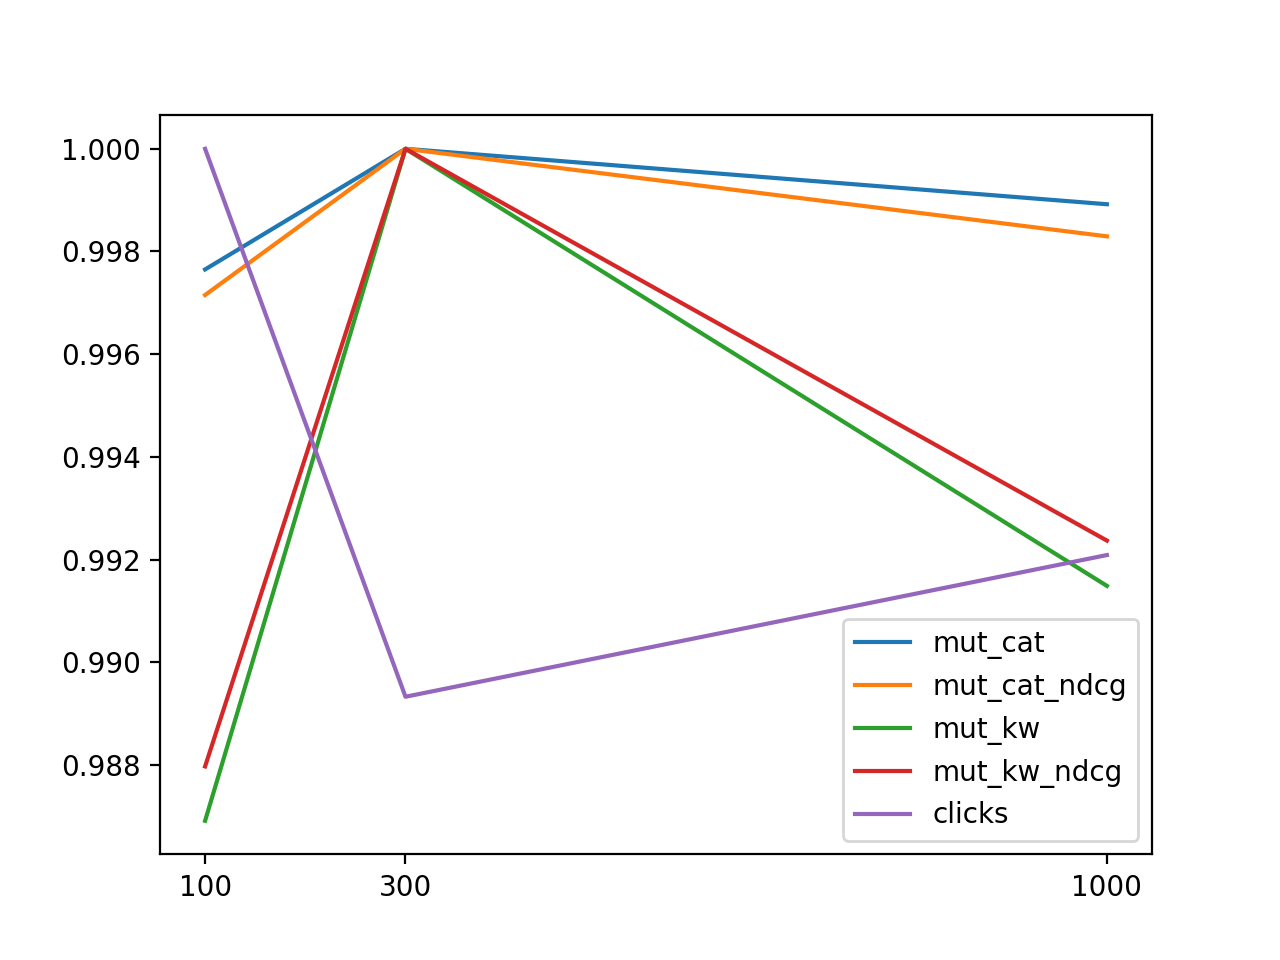
\includegraphics[width=1\textwidth]{img/results/w2v_ctr.png}
	\caption{Porównanie znormalizowanych wyników dla metody Word2vec w zależnosci od bazowego korpusu.}
	%\label{fig:warstwy}
\end{figure}

Dla różnej wymiarowości wektorów wyjściowych metoda Word2vec daje bardzo podobne rezultaty. Różnica między najlepszym i najgorszym wynikiem wynosi jedynie ok 1,5 pkt. proc. Mimo to najlepszą wartością hiperparametru wydaje się być 300.

\subsection{GloVe}

\begin{table}[H]
	\centering
	\begin{tabular}{lrrr}
		\hline
		&      100 &      300 &     1000 \\
		\hline
		mut\_cat      & 3.4595   & 3.4595   & 3.54532  \\
		mut\_cat\_ndcg & 0.510077 & 0.510077 & 0.523677 \\
		mut\_kw       & 1.79875  & 1.79875  & 2.15176  \\
		mut\_kw\_ndcg  & 0.097138 & 0.097138 & 0.115149 \\
		clicks       & 0.907997 & 0.907997 & 0.879786 \\
		\hline
	\end{tabular}
	\caption{Wyniki ewaluacji metody GloVe dla zmiennej długości wektorów.}
\end{table}

\begin{figure}[H]
	\centering
	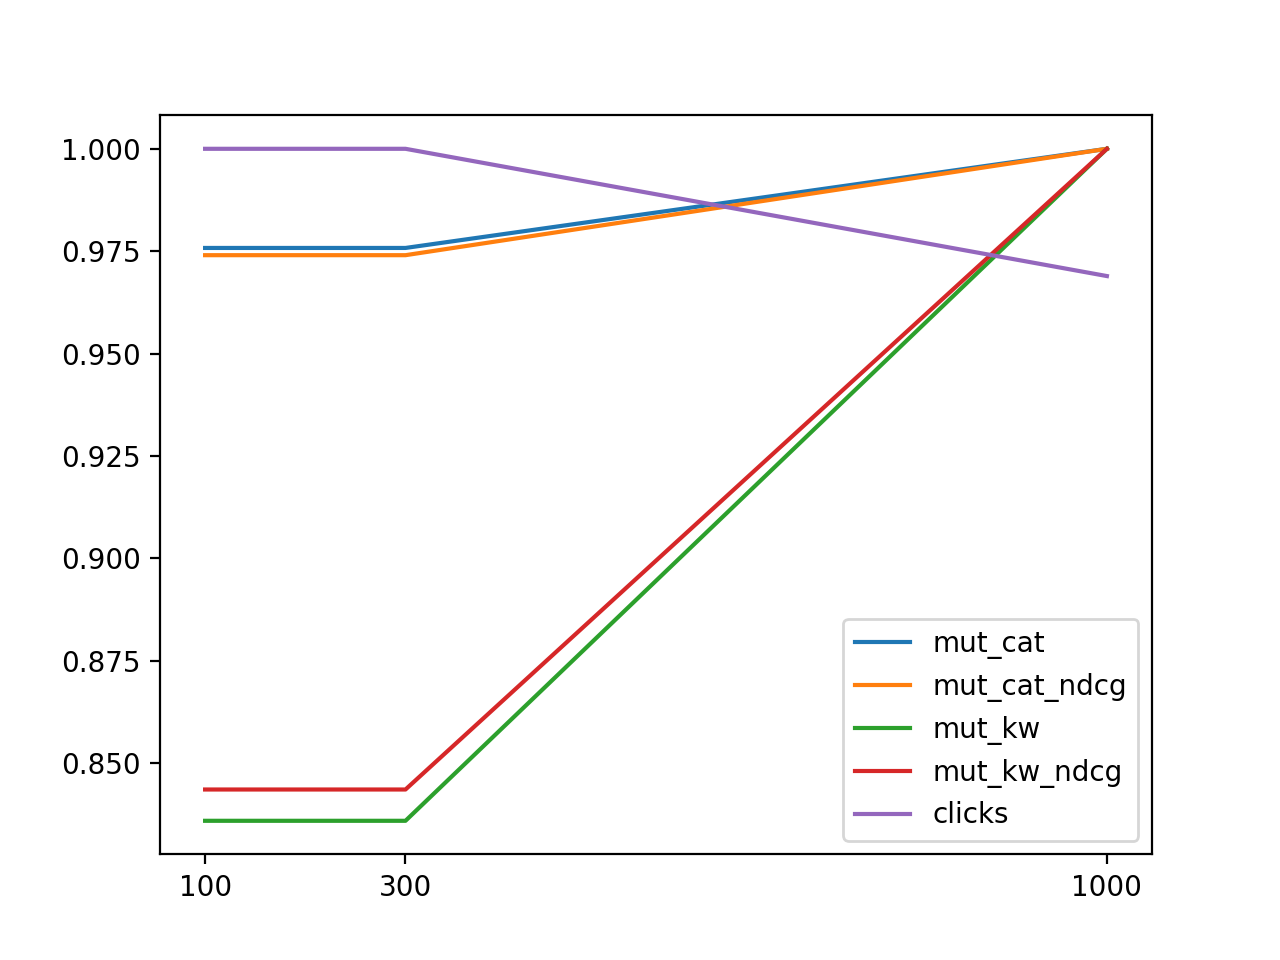
\includegraphics[width=1\textwidth]{img/results/gv_ctr.png}
	\caption{Porównanie znormalizowanych wyników dla metody GloVe w zależnosci od bazowego korpusu.}
	%\label{fig:warstwy}
\end{figure}

Ewidentnie najlepsze wyniki metoda osiąga dla wektorów wyjściowych długości 1000.

\subsection{FastText}

\begin{table}[H]
	\centering
	\begin{tabular}{lrrr}
		\hline
		&      100 &      300 &     1000 \\
		\hline
		mut\_cat      & 3.55494  & 3.57287  & 3.57869  \\
		mut\_cat\_ndcg & 0.525164 & 0.528378 & 0.528948 \\
		mut\_kw       & 2.00994  & 2.11828  & 2.16992  \\
		mut\_kw\_ndcg  & 0.108461 & 0.113908 & 0.116528 \\
		clicks       & 0.896766 & 0.89745  & 0.885622 \\
		\hline
	\end{tabular}
	\caption{Wyniki ewaluacji metody FastText dla zmiennej długości wektorów.}
\end{table}

\begin{figure}[H]
	\centering
	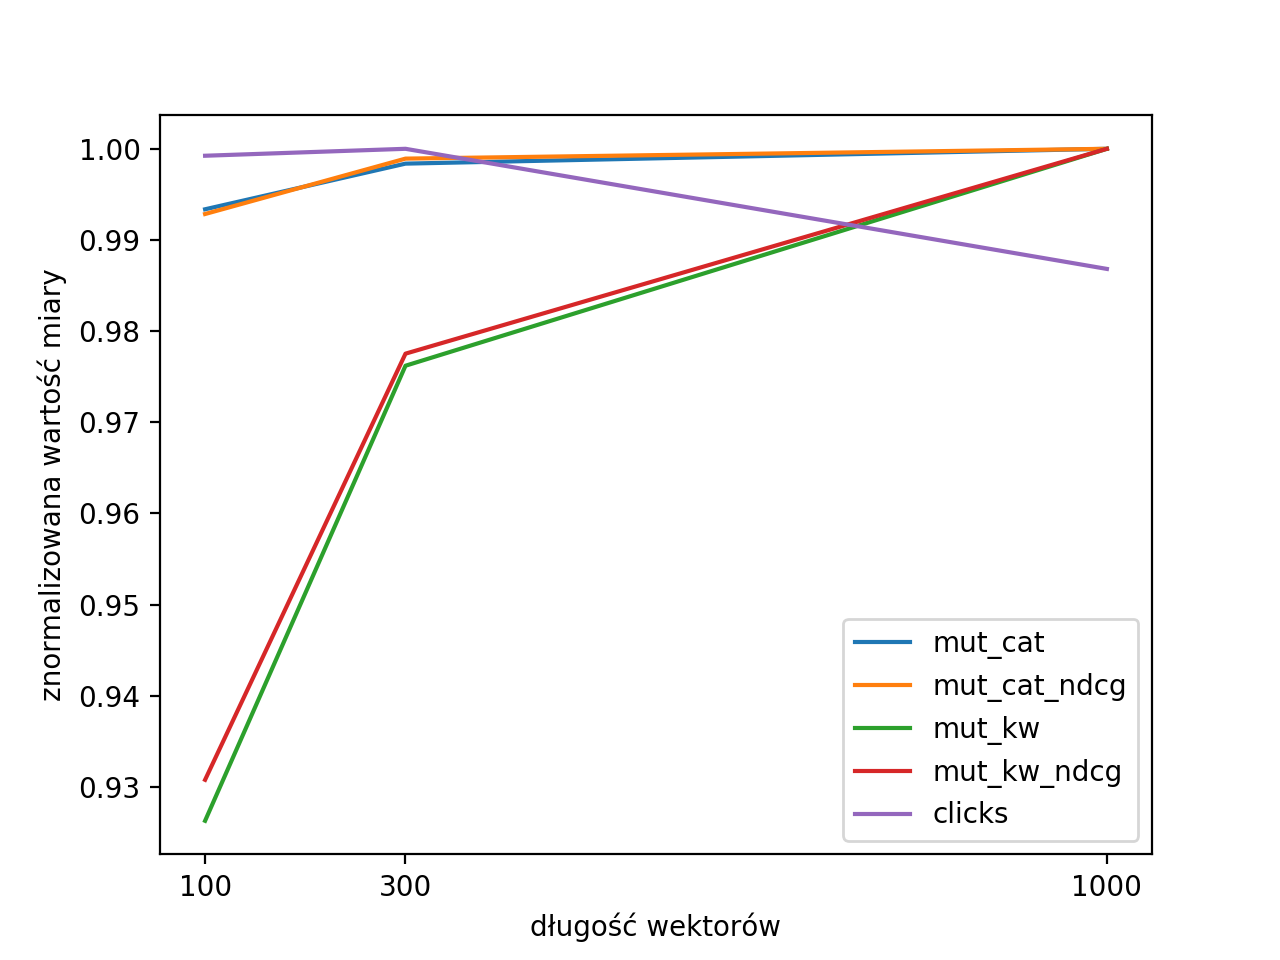
\includegraphics[width=1\textwidth]{img/results/ft_ctr.png}
	\caption{Porównanie znormalizowanych wyników dla metody FastText w zależnosci od bazowego korpusu.}
	%\label{fig:warstwy}
\end{figure}

Również jak w przypadku metody GloVe metoda FastText osiąa najlepsze rezultaty dla wektorów długości 1000.

\section{Ocena jakości wybranych metod przez użytkowników}

W niniejszym punkcie dokonuję porównania najlepszych konfiguracji testowanych wcześniej metod. Zestawiam z nimi wyniki dla metody używanej dotyczczas w Allegro oraz metodę losową.
Testowane warianty:
\begin{itemize}
	\item $lsi500$ --- Latent Semantic Indexing dla 500 tematów,
	\item $lda900$ --- Latent Dirichlet Allocation dla 900 tematów,
	\item $w2v300$ --- Word2vec dla wektorów dł. 300 i przy użytej metodzie centroidu,
	\item $w2v300$ --- GloVe dla wektorów dł. 1000 i przy użytej metodzie centroidu,
	\item $w2v300$ --- FastText dla wektorów dł. 1000 i przy użytej metodzie centroidu,
	\item $allegro$ --- używane dotychczas w Allegro zapytanie do silnika Elasticsearch,
	\item $rnd$ --- metoda losowa.
\end{itemize}
\subsection{Zestawienie wyników testów automatycznych}
Poniżej zestawienie wyników miar automatycznych dla najlepszych wariantów testowanych wcześniej metod.
\begin{table}[H]
	\centering
	\begin{tabular}{lrrrrrrr}
		\hline
		&   lsi500 &    lda900 &    w2v300 &   gv1000 &   ft1000 &   allegro &          rnd \\
		\hline
		mut\_cat      & 3.523  & 3.400   & 3.421   & 3.545  & 3.579  &  3.471  &   1.233    \\
		mut\_cat\_ndcg & 0.518 & 0.501  & 0.505  & 0.524 & 0.529 &  0.509 &   0.185    \\
		mut\_kw       & 2.388  & 1.766   & 1.684   & 2.152  & 2.170  &  3.705  &   0.137   \\
		mut\_kw\_ndcg  & 0.129 & 0.096 & 0.091 & 0.115 & 0.116 &  0.203 &   0.008 \\
		clicks       & 0.913 & 0.9064  & 0.936  & 0.880 & 0.886 &  0.890 & ---          \\
		\hline
	\end{tabular}
	\caption{Zestawienie wyników testów automatycznych dla najlepszych konfiguracji wybranych metod.}
\end{table}

\begin{figure}[H]
	\centering
	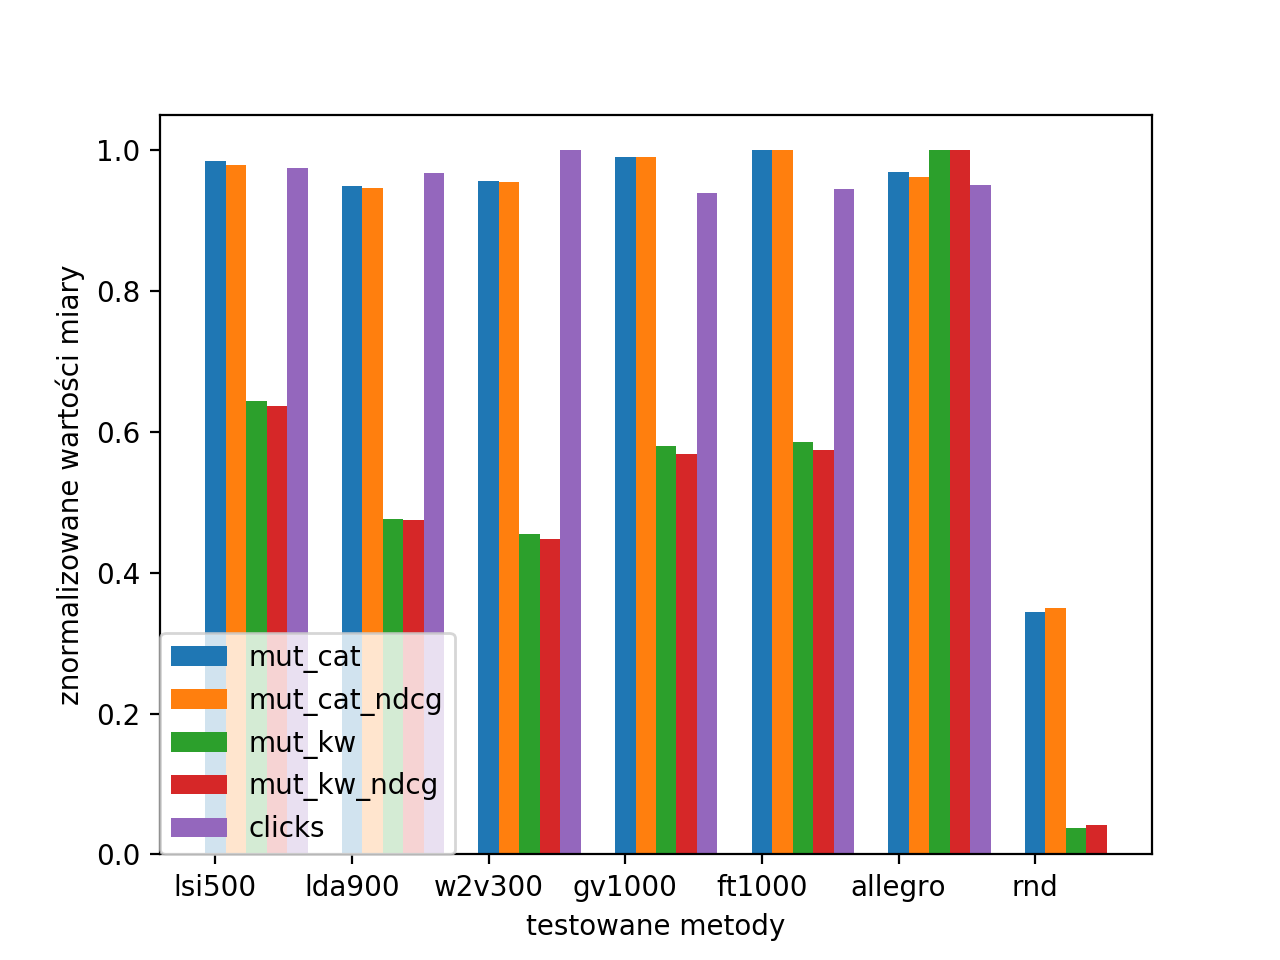
\includegraphics[width=1\textwidth]{img/results/lsi500_lda900_w2v300_gv1000_ft1000_allegro_rnd_.png}
	\caption{Porównanie znormalizowanych wyników dla wybranych metod.}
	%\label{fig:warstwy}
\end{figure}

Wszystkie testowane metody dają dużo lepsze rezultaty od metody losowej. Stasunkowo wysokie wskaźniki $mut\_cat$ dla metody losowej wynikają z dużo większej szansy, że dwa artykuły mają wspólnych przodków w drzewie kategorii niż, że mają wspólne słowa kluczowe.

Najwyższe wyniki wszystkich miar uzyskała metoda $allegro$. Jej wysokie wskaźniki dla metody $mut_kw$ wynikają wprost ze struktury zapytania do silnika Elasticsearch, które to jest oparte właśnie o słowa kluczowe dołączone do artykułu.

\subsection{Wyniki oceny eksperckiej}

\begin{table}[H]
	\centering
	\begin{tabular}{lrrrrrrr}
		\hline
		&   lsi500 &   lda900 &   w2v300 &   gv1000 &   ft1000 &   allegro &   rnd \\
		\hline
		users &    8.415 &    7.895 &    8.185 &     8.61 &     8.68 &      8.47 & 1.345 \\
		\hline
	\end{tabular}
	\caption{Zestawienie wyników ewaluacji eksperckiej dla najlepszych konfiguracji wybranych metod.}
\end{table}

\begin{figure}[H]
	\centering
	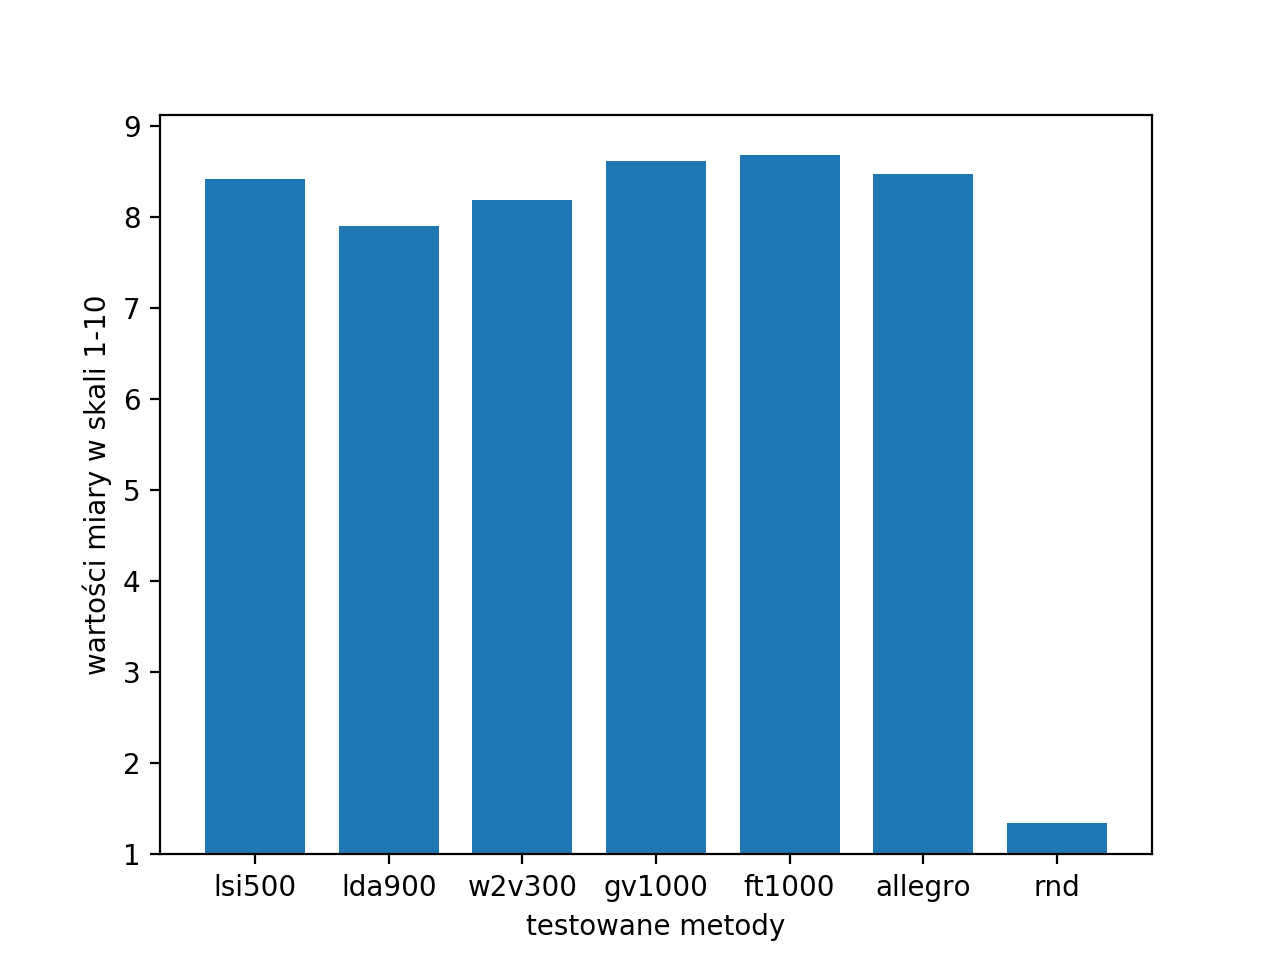
\includegraphics[width=1\textwidth]{img/results/lsi500_lda900_w2v300_gv1000_ft1000_allegro_rnd_users.png}
	\caption{Porównanie wyników ewaluacji eksperckiej dla wybranych metod.}
	%\label{fig:warstwy}
\end{figure}

Ewaluacja ekspercka wprost pokazuje, że zadna z testowanych metod nie odbiega znacząco od innych. Żadna z testowanych adaptacji metod semantycznej analizy tekstu nie odbiega róznież od dotychczasowej metody używanej w Allegro. Różnica pomiędzy najlepszą metodą (FastText) i najgorszą (LDA) wynosi ok. 9%.

Każda z testowanych metod dała również wynika znacząco lepszy od metody losowej.


\begin{table}[H]
	\centering
	\begin{tabular}{lrrrrrrr}
		\hline
		&   lsi500 &   lda900 &   w2v300 &   gv1000 &   ft1000 &   allegro &     rnd \\
		\hline
		users\_std &   2.6931 &  2.71551 &  2.59823 &  2.18813 &  2.06097 &    2.4019 & 1.34014 \\
		\hline
	\end{tabular}
	\caption{Zestawienie odchyleń standardowych ocen dokonanych przy ewaluacji eksperckiej dla najlepszych konfiguracji wybranych metod.}
\end{table}

\begin{figure}[H]
	\centering
	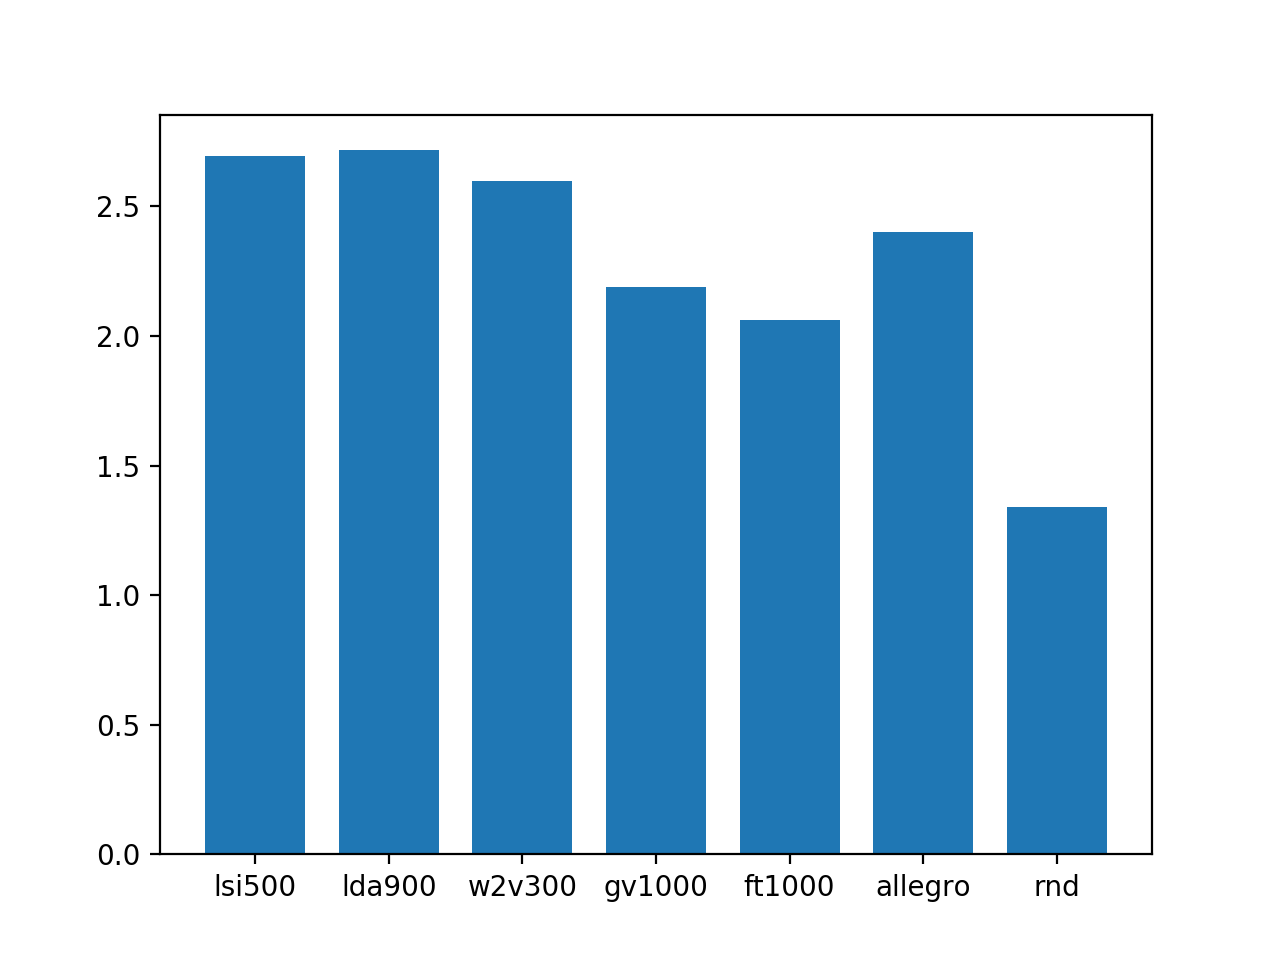
\includegraphics[width=1\textwidth]{img/results/lsi500_lda900_w2v300_gv1000_ft1000_allegro_rnd_users_std.png}
	\caption{Porównanie odchyleń standardowych ocen eksperckich dla wybranych metod.}
	%\label{fig:warstwy}
\end{figure}

Pożądaną cechą dla metody jest, aby możliwie rzadko generowała ona wyniki odstające --- w żaden sposób niezwiązane z artykułem bazowym. Stąd niska wartość odchylenia standardowego działa na korzyść metody. Tutaj również najlepszy rezultat --- najbardziej spójne wyniki uzyskała metoda FastText, nastomias najgorszy wynik znów uzyskała metoda LDA.

W świetle powyższych wyników najlepsze rezultaty zdaje się osiągać FastText. Zakładam, iż jest to związane z wewnętrzną analizą słów, jaką wykonuje ta metoda. Może się to sprawdzać szczegónie dobrze w przypadku języka polskiego, który jest językiem bogatym morfosyntaktycznie.

\section{Podsumowanie testów}

Przeprowadzone testy automatyczne miały na celu sprawdzenie, jak jakość danej metody zależy od jej konfiguracji. W tym celu wykorzystałem autorskie metody ewaluacji. W wielu przypadkach dało się zauważyć korelację między metodami ewaluacji opartymi o metadane artykułów: słowa kluczowe i kategorie.

Wartościowym okazało się rozróżnienie na ewaluację poprzez obliczenie średniej relewantności oraz obliczenie miary nDCG. Pokazało to, wyjątkowo dobrą zdolność metody WMD do poprawnego szeregowania rekomendowanych artykułów.

Wyniki metody $clicks$ --- opartej o historyczną aktywność użytkownikow --- odstają niekiedy od innych wyników. Może się to wiązać z faktem, iż liczba przejść dokonanych przez użytkowników między parami artykułów niekoniecznie odzwierciedla podobieństwo między nimi. Fakt, iż użytkownik przechodzi z artykułu $A$ do rekomendowanego artykułu $B$ może również wynikać z faktu, iż artykuł $B$ porusza inną tematykę niż artykuł $A$, która to jednak interesuje użytkownika. Wprowadznie do rekomendacji małego odsetka niepowiązanych przedmiotów jest znaną praktyką przy tworzeniu systemów rekomendacji i ma na celu zainteresowanie użytkownika przedmiotami spoza kręgu jego dotychczasowych zainteresowań.

Jakość autorskich automatycznych metod ewaluacji zdaje się potwierdzać dodadnia korelacja z wymikami oceny eksperckiej. Ocena ta pozwoliła wyznaczyć metodę najlepiej nadającą się do zadania rekomendacji artykułów w jezyku polskim oraz pokazała, że wszystkie testowane metodyw swoich najlepszych konfiguracjach dają wyniki o podobnej jakości. 


\chapter{Podsumowanie pracy i kierunki dalszych badań}
%TOTO na początku pracy zaać pytania i w podsumowaniu na nie odpowiedzieć

W niniejszej pracy starałem się sprawdzić, czy metody semantycznej analizy tekstu zaadaptowane w celu wyznaczania artykułów najbardziej podobnych do danego są w stanie dorównać dotychczas używanej w serwisie Allegro metodzie opartej o zapytanie do silnika wyszukiwania Elasticsearch. W tym celu wykonałem szereg testów sprawdzających jakość wygenerowanych rekomendacji w zależności od konfiguracji poszczególnych metod. Po analizie wyników testów można udzielić odpowiedzi: tak, każda z testowanych metod semantycznej analizy języka naturalnego w swojej najlepszej konfiguracji może zostać zaadaptowana w celu generowania rekomendacji artykułów w oparciu o treść artykułu aktualnie wyświetlanego przez użytkownika serwisu. Rekomendacje te w ocenie  użytkowników nie ustępują jakością dotychczasowej metodzie. 

Użycie metod semantycznej analizy tekstu pozwala wychwycić ukryte podobieństwa między dokumentami, gdzie dokumenty łączą nie te same słowa, czy synonimy, ale pewne złożone abstrakcyjne koncepty powiązane ze sobą. Użycie metod semantycznej analizy tekstu zwalnia autorów artykułów z samodzielnego opatrywania ich dodatkowymi słowami kluczowymi, gdyż metody te pozwalają wykazać podobieństwo w oparciu jedynie o treść dokumentu.

Istotną zaletą dotychczasowego rozwiązainia stosowanego w Allegro jest uniwersalność silnika Elasticsearch oraz to, że pozwala edytować indeksowane dane w locie, bez konieczności przebudowy systemu. Metody semantycznej analizy tekstu potrzebują przebudowania modelu przy każdej zmianie korpusu, na którym się opierają --- jest to ich istotna wada.


\section{Dalsze badania}

Analiza zawarta w tej pracy nie wyczerpuje całkowicie zagadnień związanych z tematem pracy. Przeprowadzone w pracy badania dają jedynie ogólny pogląd, ale pokazują, że istnieje pole do dalszych badań w tym kierunku.

Nietrywialnym problemem okazało się zadanie ewaluacji systemu rekomendacyjnego. Warto zaznaczyć tu różnicę pomiędzy tematyką pracy a komercyjnym zagadnieniem najlepszych rekomendacji. Artykuły najbardziej podobne wcale nie muszą być tymi, które najlepiej nadają się na rekomendacje. Otwartym pytaniem pozostaje, czy rekomendowanie użytkownikowi podobnych artykułów wprost przekłada się na zwiększenie liczby transakci zawartych przez niego. Powszechnym zjawiskiem jest wzbogacanie rekomandacji o przedmioty niepodobne do danego, a pozwalające użytkownikowi na poznanie osobnej kategorii przedmiotów, która może go zainteresować a tym samym przyciągnąć do serwisu. Ostatecznym celem użycia systemu rekomendacji jest w dłuższej perspektywie maksymalizacja zysku serwisu przez kierowanie użytkowników na strony ofert, co zwiększa szansę a dokonanie przez nich transakcji. Trudność oceny jakości takiego systemu wiąże się z mnogością czynników, które kierują zachowaniami użytkowników. Dopiero badania na ,,żywym systemie'' są w stanie wykazać realną wyższość jednej z metod nad innymi. Sporządzenie systemu rekomandacji uwzględniającego te czynniki wydaje się więc być osobnym tematem godnym szczegółowych badań.

Przed zastosowaniem metod wyznaczania podobieństwa wykonałem przetwarzanie wstępne dokumentów, które można przeprowadzić również na inne sposoby. Dobór metod wstępnego przetwarzania tekstu jest zawsze kwestią indywidalną, trudną w ocenie.

Innym aspektem jest założenie braku dynamiki systemu. Konieczność przebudowywania modelu przy każdej zmianie w bazie artykułów w praktyce mogłaby powodować niemożność zastosowania metod semantycznej analizy tekstu w tym celu. Tempo zmian rzeczywistego zbioru artykułów oraz czasy budowania modeli nie były poruszane w niniejszej pracy.

Można by zastosować inne metody wyznaczania odległości między wektorowymi reprezentacjami dokumentów. Metoda centroidu jest szybka i prosta, ale dokonuje sporego uproszczenia struktury dokumentu. Metoda WMD daje natomiast lepsze uszeregowanie, ale kosztem dużej złożoności obliczeniowej.
%Inne ciekawe badania w tym temacie
%Kwestie, które wykraczają poza zakres niniejszej pracy, a są związane z jej tematyką
%Otrzymane wyniki nie wskazują jednoznacznej przewagi jednej metody nad innymi.

\begin{thebibliography}{30}
	\bibitem{allegro}
		Opis Allegro
		\url{https://magazyn.allegro.pl/3333-serwis-allegro-to-nasz-sposob-na-wasze-szybkie-i-wygodne-zakupy-przez-internet}
		(dostęp 07.05.2017)
	
	\bibitem{bengio}
		Y. Bengio, R. Ducharme, P. Vincent, C. Jauvin,
		\emph{A Neural Probabilistic Language Model},
		Journal of Machine Learning Research 3 1137–1155,
		2003
	
	\bibitem{lda}
		D. M. Blei, A. Y. Ng, M. I. Jordan,
		\emph{Latent Dirichlet Allocation},
		Journal of Machine Learning Research, tom 3 num. 4–5,
		2003
		
	\bibitem{aylien}
		Blog Aylien
		\url{http://blog.aylien.com/overview-word-embeddings-history-word2vec-cbow-glove/}
		(dostęp 18.08.2017)
	
	\bibitem{c_w}
		R. Collobert, J. Weston,
		\emph{A Unified Architecture for Natural Language Processing: Deep Neural Networks with Multitask Learning},
		NEC Labs America,
		2008
	
	\bibitem{lsa}
		S. Deerwester, S. T. Dumais, G. W. Furnas, T. K. Landauer, R. Harshman,
		\emph{Indexing by latent semantic analysis},
		Journal of the American Society for Information Science, tom 41, num. 6,
		1990
	
	\bibitem{elastic}
		Elasticsearch
		\url{https://www.elastic.co/}
		(dostęp 18.08.2017)
	
	\bibitem{elastic_companies}
		Firmy korzystające z Elasticsearch
		\url{https://www.elastic.co/use-cases}
		(dostęp 10.08.17)
	
	\bibitem{firth}
		J.R. Firth,
		\emph{A synopsis of linguistic theory 1930-1955},
		Oxford: Philological Society,
		1957
	
	\bibitem{svd}
		G. H. Golub, W. Kahan,
		\emph{Calculating the singular values and pseudo-inverse of a matrix},
		Journal of the Society for Industrial and Applied Mathematics: Series B, Numerical Analysis. 2 (2),
		1965
	
	\bibitem{bow}
		Z. S. Harris,
		\emph{Distributional Structure},
		WORD, tom 10, num. 2-3,
		1954
	
	\bibitem{google_word2vec}
		Informacje o Word2vec
		\url{https://code.google.com/archive/p/word2vec/}
		(dostęp 26.05.2017)
	
	\bibitem{ndcg}
		K. Jarvelin, J. Kekalainen,
		\emph{Cumulated gain-based evaluation of IR techniques},
		University of Tampere,
		2002
	
	\bibitem{fasttext}
		A. Joulin, E. Grave, P. Bojanowski T. Mikolov,
		\emph{Bag of Tricks for Efficient Text Classification},
		Facebook AI Research,
		2016
	
	\bibitem{pias}
		P. Kędzia, G. Czachor, M. Piasecki, J. Kocoń
		\emph{Vector representations of polish words (Word2Vec method)},
		Wrocław University of Technology,
		2016,
		\url{https://clarin-pl.eu/dspace/handle/11321/327}
		(dostęp 26.06.2017)
	
	\bibitem{wmd}
		M. J. Kusner, Y. Sun, N. I. Kolkin, K. Q. Weinberger,
		\emph{From Word Embeddings To Document Distances},
		International Conference on Machine Learning (ICML),
		2015
	
	\bibitem{lucene}
		Lucene
		\url{https://lucene.apache.org/}
		(dostęp 18.08.2017)
	
	\bibitem{word2vec}
		T. Mikolov, K. Chen, G. Corrado, J. Dean,
		\emph{Efficient Estimation of Word Representations in Vector Space},
		International Conference on Machine Learning (ICML),
		2013
	
	\bibitem{morfologik}
		Morfologik
		\url{http://morfologik.blogspot.com/}
		(dostęp 07.05.2017)
	
	\bibitem{glove_cran}
		Opis GloVe
		\url{https://cran.r-project.org/web/packages/text2vec/vignettes/glove.html}
		(dostęp 30.08.2017)
	
	\bibitem{word2vec_tutorial}
		Opis Word2vec
		\url{http://mccormickml.com/2016/04/19/word2vec-tutorial-the-skip-gram-model/}
		(dostęp 26.05.2017)
	
	\bibitem{emd_method}
		O. Pele, M. Werman,
		\emph{Fast and robust earth mover's distances},
		ICCV,
		2009
	
	\bibitem{glove}
		J. Pennington, R. Socher, C. D. Manning,
		\emph{GloVe: Global Vectors for Word Representation},
		Computer Science Department, Stanford University, Stanford, CA 94305,
		2014
	
	\bibitem{all_naj}
		Porównanie największych polskich serwisów aukcyjnych
		\url{http://gadzetomania.pl/11824,zakupy-w-sieci-porownanie-najwiekszych-polskich-serwisow-aukcyjnych-2}
		(dostęp 09.08.17)
	
	\bibitem{handbook}
		F. Ricci, L. Rokach, B. Shapira,
		\emph{Introduction to Recommender Systems Handbook},
		Springer,
		2011
	
	\bibitem{emd}
		Y. Rubner, C. Tomasi, L. J. Guibas,
		\emph{The Earth Mover's Distance as a Metric for Image Retrieval},
		str. 1,
		Computer Science Department, Stanford University,
		2000	

	\bibitem{tf_idf}
		G. Salton and M. McGill,
		\emph{Introduction to modern information retrieval},
		McGraw-Hill,
		1983
	
	\bibitem{stopwords}
		Słowa stopu w Wikipedii
		\url{https://pl.wikipedia.org/wiki/Wikipedia:Stopwords}
		(dostęp 15.04.2017)
	
	\bibitem{slownik}
		Słownik Języka Polskiego PWN
		\url{http://sjp.pwn.pl/sjp/artykul;2441396.html}
		(dostęp 07.05.2017)
	
	\bibitem{screen_allegro}
		Strona Allegro z artykułem
		\url{https://allegro.pl/artykul/jaka-farba-dla-alergika-55917/}
		(dostęp 26.06.2017)
		
	\bibitem{wordnet}
		Wordnet
		\url{http://plwordnet.pwr.wroc.pl/wordnet/}
		(dostęp 28.06.2017)
\end{thebibliography}



% 7. Wykaz symboli i skrótów - jeśli nie ma, zakomentować
%\chapter*{Wykaz symboli i skrótów}

%\begin{tabular}{cl}
%nzw. & nadzwyczajny \\
%* & operator gwiazdka \\
%$\widetilde{}$ & tylda
%\end{tabular}


% 8. Spis rysunków - jeśli nie ma, zakomentować (ale być może po prostu się nie zrobi)
\listoffigures


% 9. Spis tabel - jak wyżej
\renewcommand{\listtablename}{Spis tabel}
\listoftables


% 10. Spis załączników - jak nie ma załączników, to zakomentować lub usunąć
\chapter*{Spis załączników}
\begin{enumerate}
\item[1.] Wykorzystane technologie i narzędzia
\item[2.] Zawartość dołączonej płyty CD
\end{enumerate}

% 11. Załączniki
\newpage
\pagestyle{empty}
\appendix
\chapter{Wykorzystane technologie i narzędzia}
Analizę danych, ich wstępne przetworzenie a następnie przeprowadzenie docelowych eksperymentów wykonałem korzystając głównie z języka Python i szeregu skrytpów napisanych w nim własnoręcznie, wykorzystujących istniejące specjalistyczne biblioteki posiadające interfejs w tymże języku.

Wykorzystane narzędzia:
\begin{itemize}
	\item Elasticsearch --- silnik wyszukiwania tekstowego. Używam go do przechowywania bazy artykułów oraz ich przetworzonych wersji.
	\item MongoDB --- nierelacyjna baza danych, której używam do przechowywania wyników generowanych przez testowane algorytmy.
	\item GloVe --- implementacja metody GloVe. Generuje wektory słów, które następnie mogą być wykorzystane np. przez bibliotekę gensim.
	\item FastText --- implementacja metody FastText wykonana przez zespół Facebook Research. Generuje wektory słów, które następnie mogą być wykorzystane np. przez bibliotekę gensim.
\end{itemize}

Poniższa lista zawiera wykorzystane biblioteki języka Python:
\begin{itemize}
	\item Gensim --- rozbudowana biblioteka służąca do przetwarzania języka naturalnego; zawiera implementację metod Word2Vec, LSI, LDA, TF-IDF i inne.
	\item Morfologik --- tokenizer języka polskiego.
	\item Numpy --- pozwala wydajnie wykonywać obliczenia numeryczne.
	\item Pyemd --- implementacja algorytmu Earth Mover's Distance.
	\item Elasticsearch --- ułatwia wykonywanie zapytań do silnika Elasticsearch wprost z kodu Pythona.
	\item Matplotlib --- biblioteka służąca do wykonywania wykresów.
	\item Pymongo --- umożliwia wykonywanie zapytań do bazy MongoDB wprost z kodu Pythona.
\end{itemize}

\chapter{Zawartość dołączonej płyty CD}
%TODO w dodaktu opisać zawartość dołączonej płyty
\end{document}